\subsubsection{Engineer Use Cases}
The Engineer actor focuses on training path enrollment, virtual lab access, and
hands-on learning. The key use cases include training path enrollment and management,
content consumption (videos, articles, quizzes), virtual machine session management,
hardware device and camera control, reservation management, forum participation,
certificate claims, payment operations, and account management.
 
\subsubsubsection[Follow Training Paths]{Refinement of the Use Case Follow Training Paths} Figure
\ref{fig:eng-follow-training-paths-use-case} presents the refinement of the
Use Case Follow Training Paths for the Engineer actor. This use case includes
the following sub-use cases:
\begin{figure}[H]
    \centering
    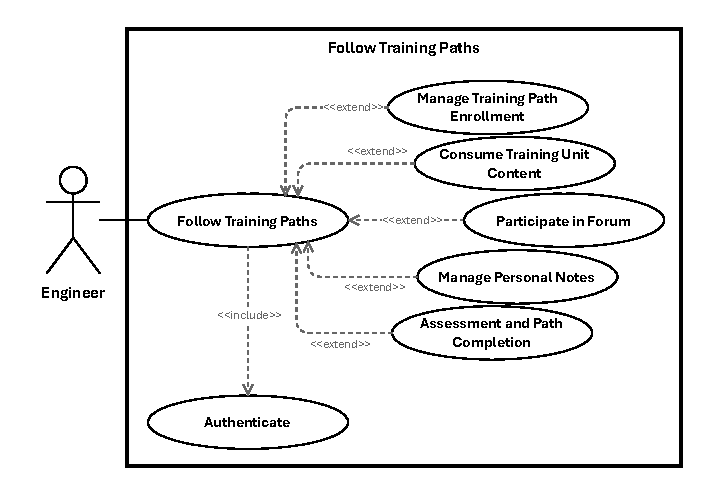
\includegraphics[width=\textwidth]{assets/chapter3/eng-follow-training-paths-use-case}
    \caption{Use Case Follow Training Paths}
    \label{fig:eng-follow-training-paths-use-case}
\end{figure}
%% ─── FOLLOW TRAINING PATHS ───────────────────────────────────────────────────

\dotsection{\textbf{Specification of the Use Case Manage Training Path Enrollment}}
\begin{table}[H]
    \centering
    \caption{Use Case Specification: Manage Training Path Enrollment}
    \begin{tabular}{|p{3.5cm}|p{10.5cm}|}
        \hline
        \textbf{Title}          & Manage Training Path Enrollment \\
        \hline
        \textbf{Summary}        & Engineer browses their enrolled training paths, enrolls in new ones, and unenrolls from paths they no longer wish to pursue \\
        \hline
        \textbf{Actor}          & Engineer \\
        \hline
        \textbf{Precondition}   & The engineer is authenticated and the target training path is published and available where applicable \\
        \hline
        \textbf{Post-condition} & The engineer's enrollment state is created or removed and access to training path content is granted or revoked accordingly \\
        \hline
        \textbf{Basic Scenario} & \begin{minipage}[t]{\linewidth}
            \begin{enumerate}[topsep=0pt,itemsep=1pt,parsep=0pt,partopsep=0pt]
                \item Engineer opens the dashboard; system displays all enrolled training paths with title, thumbnail, progress percentage, and status; engineer may filter by status or category
                \item For \textbf{Enroll}: engineer selects a training path from the catalog and clicks Enroll; if the path is free enrollment is immediate; if paid the engineer is redirected to checkout; upon success the system creates the enrollment record and grants access to all modules and units
                \item For \textbf{Unenroll}: engineer selects an enrolled training path and confirms the unenrollment action; system removes the enrollment record, revokes content access, and handles any applicable refund according to platform policy
            \end{enumerate}
        \end{minipage} \\
        \hline
        \textbf{Error Scenario} & \begin{minipage}[t]{\linewidth}
            \begin{enumerate}[topsep=0pt,itemsep=1pt,parsep=0pt,partopsep=0pt]
                \item If the engineer has no enrollments, system displays an empty state with discovery suggestions
                \item If the engineer is already enrolled, system displays a message and prevents duplicate enrollment
                \item If the training path is unpublished or archived, enrollment is blocked and the path is marked accordingly
                \item If payment fails, enrollment is not completed
                \item If unenrollment is restricted due to completion status, system displays an explanatory message
            \end{enumerate}
        \end{minipage} \\
        \hline
    \end{tabular}
    \label{tab:eng-enrollment}
\end{table}

\dotsection{\textbf{Specification of the Use Case Consume Training Unit Content}}
\begin{table}[H]
    \centering
    \caption{Use Case Specification: Consume Training Unit Content}
    \begin{tabular}{|p{3.5cm}|p{10.5cm}|}
        \hline
        \textbf{Title}          & Consume Training Unit Content \\
        \hline
        \textbf{Summary}        & Engineer watches video lessons, reads article lessons, and marks training units complete or incomplete, with progress tracked and persisted throughout \\
        \hline
        \textbf{Actor}          & Engineer \\
        \hline
        \textbf{Precondition}   & The engineer is enrolled in the training path and the target training unit is accessible and published \\
        \hline
        \textbf{Post-condition} & The engineer's content progress is recorded and the overall training path progress is recalculated accordingly \\
        \hline
        \textbf{Basic Scenario} & \begin{minipage}[t]{\linewidth}
            \begin{enumerate}[topsep=0pt,itemsep=1pt,parsep=0pt,partopsep=0pt]
                \item Engineer opens a training unit from their enrolled training path
                \item For \textbf{Video}: system loads the video player with the processed stream URL; engineer plays, pauses, seeks, or adjusts playback speed; system periodically records playback position; upon reaching the completion threshold the video is marked as watched
                \item For \textbf{Article}: system renders the article with estimated reading time; engineer scrolls through the content; system tracks progress via scroll position or explicit confirmation; upon reaching the end the article is marked as read
                \item Engineer may manually \textbf{mark the unit complete or incomplete} at any time; system persists the status and recalculates module and path-level progress percentages
                \item Updated progress is reflected on the training path overview
            \end{enumerate}
        \end{minipage} \\
        \hline
        \textbf{Error Scenario} & \begin{minipage}[t]{\linewidth}
            \begin{enumerate}[topsep=0pt,itemsep=1pt,parsep=0pt,partopsep=0pt]
                \item If the video has not finished processing, system displays a pending state with a retry option
                \item If the video stream URL is unavailable, system shows an error with a fallback message
                \item If the article is unpublished or fails to load, system shows a notice and prevents access
                \item If progress saving fails, system retries silently and preserves the last known state
                \item If the engineer is not enrolled, system denies access and progress updates
            \end{enumerate}
        \end{minipage} \\
        \hline
    \end{tabular}
    \label{tab:eng-consume-content}
\end{table}

\dotsection{\textbf{Specification of the Use Case Participate in Forum}}
\begin{table}[H]
    \centering
    \caption{Use Case Specification: Participate in Forum}
    \begin{tabular}{|p{3.5cm}|p{10.5cm}|}
        \hline
        \textbf{Title}          & Participate in Forum \\
        \hline
        \textbf{Summary}        & Engineer engages with training path discussion forums by posting threads or replies, upvoting helpful content, and flagging inappropriate content for moderation \\
        \hline
        \textbf{Actor}          & Engineer \\
        \hline
        \textbf{Precondition}   & The engineer is enrolled in at least one training path with an active forum \\
        \hline
        \textbf{Post-condition} & The engineer's post, upvote, or flag is persisted and reflected in the forum accordingly \\
        \hline
        \textbf{Basic Scenario} & \begin{minipage}[t]{\linewidth}
            \begin{enumerate}[topsep=0pt,itemsep=1pt,parsep=0pt,partopsep=0pt]
                \item Engineer navigates to the forum section of an enrolled training path
                \item For \textbf{Post}: engineer creates a new discussion thread or replies to an existing post; system validates content, persists the post, and notifies subscribed participants
                \item For \textbf{Upvote}: engineer clicks the upvote button on a thread or reply; system increments the upvote count and records the vote; engineer may remove their upvote at any time
                \item For \textbf{Flag}: engineer clicks the flag button to report inappropriate content; system records the flag and may hide the content pending moderator review; engineer may remove their flag if desired
            \end{enumerate}
        \end{minipage} \\
        \hline
        \textbf{Error Scenario} & \begin{minipage}[t]{\linewidth}
            \begin{enumerate}[topsep=0pt,itemsep=1pt,parsep=0pt,partopsep=0pt]
                \item If the forum is closed or locked, system prevents new posts and replies
                \item If content validation fails, system displays specific error messages and preserves input
                \item If the engineer has already upvoted, system prevents duplicate votes
                \item If the content has already been flagged, system acknowledges the existing report
            \end{enumerate}
        \end{minipage} \\
        \hline
    \end{tabular}
    \label{tab:eng-forum-participate}
\end{table}

\dotsection{\textbf{Specification of the Use Case Manage Personal Notes}}
\begin{table}[H]
    \centering
    \caption{Use Case Specification: Manage Personal Notes}
    \begin{tabular}{|p{3.5cm}|p{10.5cm}|}
        \hline
        \textbf{Title}          & Manage Personal Notes \\
        \hline
        \textbf{Summary}        & Engineer creates, edits, and deletes private notes attached to training units for personal reference \\
        \hline
        \textbf{Actor}          & Engineer \\
        \hline
        \textbf{Precondition}   & The engineer is enrolled in the training path and the training unit is accessible \\
        \hline
        \textbf{Post-condition} & The note is persisted, updated, or removed; notes remain private and are never visible to other users \\
        \hline
        \textbf{Basic Scenario} & \begin{minipage}[t]{\linewidth}
            \begin{enumerate}[topsep=0pt,itemsep=1pt,parsep=0pt,partopsep=0pt]
                \item Engineer opens a training unit; system displays any existing notes or an empty editor
                \item Engineer writes or edits note content; system validates and persists the note on save
                \item Engineer may delete a note at any time; system requests confirmation then removes it
            \end{enumerate}
        \end{minipage} \\
        \hline
        \textbf{Error Scenario} & \begin{minipage}[t]{\linewidth}
            \begin{enumerate}[topsep=0pt,itemsep=1pt,parsep=0pt,partopsep=0pt]
                \item If note content exceeds the maximum length, validation fails with a specific message
                \item If the engineer is not enrolled, system prevents note creation
                \item If save or deletion fails, system preserves the current state and logs the error
            \end{enumerate}
        \end{minipage} \\
        \hline
    \end{tabular}
    \label{tab:eng-notes}
\end{table}

\dotsection{\textbf{Specification of the Use Case Assessment and Path Completion}}
\begin{table}[H]
    \centering
    \caption{Use Case Specification: Assessment and Path Completion}
    \begin{tabular}{|p{3.5cm}|p{10.5cm}|}
        \hline
        \textbf{Title}          & Assessment and Path Completion \\
        \hline
        \textbf{Summary}        & Engineer takes quiz assessments to test knowledge, writes a course review to share feedback, and claims a completion certificate upon finishing all training path requirements \\
        \hline
        \textbf{Actor}          & Engineer \\
        \hline
        \textbf{Precondition}   & The engineer is enrolled in the training path; the quiz is published for assessment; all modules and quizzes are completed before certificate claim \\
        \hline
        \textbf{Post-condition} & Quiz attempt is recorded and scored; review is persisted and visible after approval; certificate is generated and available on the engineer's profile \\
        \hline
        \textbf{Basic Scenario} & \begin{minipage}[t]{\linewidth}
            \begin{enumerate}[topsep=0pt,itemsep=1pt,parsep=0pt,partopsep=0pt]
                \item For \textbf{Quiz}: engineer opens a training unit containing a quiz; system displays instructions, question count, and time limit; engineer answers all questions and submits or time expires; system grades the attempt, displays results with correct answers and explanations, and updates training unit progress based on passing criteria
                \item For \textbf{Review}: engineer navigates to the training path review section; selects a star rating and optionally writes a text review; system validates content, persists the review, recalculates the path average rating, and makes the review visible once approved; if a review already exists the system offers an edit option instead
                \item For \textbf{Certificate}: engineer opens the completed training path overview; system verifies all completion requirements are met, generates a unique certificate with a verification hash, and makes it available for download, sharing, and display on the engineer's public profile
            \end{enumerate}
        \end{minipage} \\
        \hline
        \textbf{Error Scenario} & \begin{minipage}[t]{\linewidth}
            \begin{enumerate}[topsep=0pt,itemsep=1pt,parsep=0pt,partopsep=0pt]
                \item If the quiz has already been attempted and retakes are not allowed, access is blocked
                \item If quiz submission fails, system preserves answers and allows retry
                \item If the rating is missing, system rejects the review submission
                \item If review text violates content policies, system flags it for moderation
                \item If completion requirements are not fully met, system displays the remaining items and blocks certificate generation
                \item If certificate generation fails, system logs the error and allows retry
            \end{enumerate}
        \end{minipage} \\
        \hline
    \end{tabular}
    \label{tab:eng-assessment-completion}
\end{table}
\iffalse
\dotsection{\textbf{Specification of the Use Case View My Enrolled Training Paths}}
\begin{table}[H]
    \centering
    \caption{Use Case Specification: View My Enrolled Training Paths}
    \begin{tabular}{|p{3.5cm}|p{10.5cm}|}
        \hline
        \textbf{Title}          & View My Enrolled Training Paths                                                              \\
        \hline
        \textbf{Summary}        & Engineer browses the list of training paths in which they are enrolled                      \\
        \hline
        \textbf{Actor}          & Engineer                                                                                    \\
        \hline
        \textbf{Precondition}   & The engineer is authenticated and has at least one enrollment                               \\
        \hline
        \textbf{Post-condition} & The engineer views a paginated list of enrolled training paths with progress indicators     \\
        \hline
        \textbf{Basic Scenario} & \begin{minipage}[t]{\linewidth}
                                      \begin{enumerate}[topsep=0pt,itemsep=1pt,parsep=0pt,partopsep=0pt]
                                          \item Engineer opens the dashboard or training paths overview
                                          \item System retrieves all training path enrollments for the authenticated user
                                          \item System displays each training path with title, thumbnail, progress percentage,
                                                and status
                                          \item Engineer may filter by status (in progress, completed) or category
                                          \item Engineer selects a training path to view its modules and units
                                      \end{enumerate}
                                  \end{minipage} \\
        \hline
        \textbf{Error Scenario} & \begin{minipage}[t]{\linewidth}
                                      \begin{enumerate}[topsep=0pt,itemsep=1pt,parsep=0pt,partopsep=0pt]
                                          \item If the engineer has no enrollments, the system displays an empty-state with
                                                discovery suggestions
                                          \item If the training path has been archived, the system marks it accordingly
                                      \end{enumerate}
                                  \end{minipage}    \\
        \hline
    \end{tabular}
    \label{tab:eng-view-enrolled}
\end{table}
\dotsection{\textbf{Specification of the Use Case Enroll in Training Path}}
\begin{table}[H]
    \centering
    \caption{Use Case Specification: Enroll in Training Path}
    \begin{tabular}{|p{3.5cm}|p{10.5cm}|}
        \hline
        \textbf{Title}          & Enroll in Training Path                                                                 \\
        \hline
        \textbf{Summary}        & Engineer enrolls in a training path to access its learning content and laboratory resources \\
        \hline
        \textbf{Actor}          & Engineer                                                                                 \\
        \hline
        \textbf{Precondition}   & The engineer is authenticated and the training path is published and available           \\
        \hline
        \textbf{Post-condition} & The engineer is enrolled in the training path and can access its modules and units       \\
        \hline
        \textbf{Basic Scenario} & \begin{minipage}[t]{\linewidth}
                                      \begin{enumerate}[topsep=0pt,itemsep=1pt,parsep=0pt,partopsep=0pt]
                                          \item Engineer browses the training path catalog
                                          \item Engineer selects a training path to view its details
                                          \item System displays training path information, syllabus, and enrollment options
                                          \item Engineer clicks the Enroll button
                                          \item If the training path is free, enrollment is immediate
                                          \item If the training path is paid, engineer is redirected to checkout
                                          \item System creates the enrollment record and grants access
                                          \item Engineer can now access the training path content
                                      \end{enumerate}
                                  \end{minipage} \\
        \hline
        \textbf{Error Scenario} & \begin{minipage}[t]{\linewidth}
                                      \begin{enumerate}[topsep=0pt,itemsep=1pt,parsep=0pt,partopsep=0pt]
                                          \item If the engineer is already enrolled, the system displays a message
                                          \item If the training path is not published, enrollment is blocked
                                          \item If payment is required and fails, enrollment is not completed
                                      \end{enumerate}
                                  \end{minipage} \\
        \hline
    \end{tabular}
    \label{tab:eng-enroll}
\end{table}
\dotsection{\textbf{Specification of the Use Case Unenroll from Training Path}}
\begin{table}[H]
    \centering
    \caption{Use Case Specification: Unenroll from Training Path}
    \begin{tabular}{|p{3.5cm}|p{10.5cm}|}
        \hline
        \textbf{Title}          & Unenroll from Training Path                                                               \\
        \hline
        \textbf{Summary}        & Engineer removes their enrollment from a training path they no longer wish to pursue       \\
        \hline
        \textbf{Actor}          & Engineer                                                                                   \\
        \hline
        \textbf{Precondition}   & The engineer is enrolled in the training path                                             \\
        \hline
        \textbf{Post-condition} & The enrollment is removed and access to training path content is revoked                 \\
        \hline
        \textbf{Basic Scenario} & \begin{minipage}[t]{\linewidth}
                                      \begin{enumerate}[topsep=0pt,itemsep=1pt,parsep=0pt,partopsep=0pt]
                                          \item Engineer navigates to their enrolled training paths
                                          \item Engineer selects the training path to unenroll from
                                          \item System displays enrollment details and unenroll option
                                          \item Engineer confirms the unenrollment action
                                          \item System removes the enrollment record
                                          \item System revokes access to training path content
                                          \item Progress and completion data may be preserved or removed according to policy
                                      \end{enumerate}
                                  \end{minipage} \\
        \hline
        \textbf{Error Scenario} & \begin{minipage}[t]{\linewidth}
                                      \begin{enumerate}[topsep=0pt,itemsep=1pt,parsep=0pt,partopsep=0pt]
                                          \item If the training path has been completed, unenrollment may be restricted
                                          \item If a refund is applicable, the system processes it according to policy
                                      \end{enumerate}
                                  \end{minipage} \\
        \hline
    \end{tabular}
    \label{tab:eng-unenroll}
\end{table}
\dotsection{\textbf{Specification of the Use Case Watch Video Lesson}}
\begin{table}[H]
    \centering
    \caption{Use Case Specification: Watch Video Lesson}
    \begin{tabular}{|p{3.5cm}|p{10.5cm}|}
        \hline
        \textbf{Title}          & Watch Video Lesson                                                                               \\
        \hline
        \textbf{Summary}        & Engineer streams an instructional video attached to a training unit and tracks playback progress \\
        \hline
        \textbf{Actor}          & Engineer                                                                                         \\
        \hline
        \textbf{Precondition}   & The engineer is enrolled in the training path and the video has been processed and published     \\
        \hline
        \textbf{Post-condition} & The engineer's video progress is recorded and the training unit progress is updated accordingly  \\
        \hline
        \textbf{Basic Scenario} & \begin{minipage}[t]{\linewidth}
                                      \begin{enumerate}[topsep=0pt,itemsep=1pt,parsep=0pt,partopsep=0pt]
                                          \item Engineer navigates to a training unit containing a video
                                          \item System loads the video player with the processed stream URL
                                          \item Engineer plays, pauses, seeks, or adjusts playback speed
                                          \item System periodically records the playback position as video progress
                                          \item When the engineer reaches the completion threshold, the system marks the video
                                                as watched
                                          \item Training unit progress is updated to reflect video completion
                                      \end{enumerate}
                                  \end{minipage}      \\
        \hline
        \textbf{Error Scenario} & \begin{minipage}[t]{\linewidth}
                                      \begin{enumerate}[topsep=0pt,itemsep=1pt,parsep=0pt,partopsep=0pt]
                                          \item If the video has not finished processing, the system displays a pending state
                                                with retry option
                                          \item If the stream URL is unavailable, the system shows an error with a fallback
                                                message
                                          \item If progress saving fails, the system retries silently and preserves the last
                                                known position
                                      \end{enumerate}
                                  \end{minipage}       \\
        \hline
    \end{tabular}
    \label{tab:eng-watch-video}
\end{table}
\dotsection{\textbf{Specification of the Use Case Read Article Lesson}}
\begin{table}[H]
    \centering
    \caption{Use Case Specification: Read Article Lesson}
    \begin{tabular}{|p{3.5cm}|p{10.5cm}|}
        \hline
        \textbf{Title}          & Read Article Lesson                                                                           \\
        \hline
        \textbf{Summary}        & Engineer reads a textual article attached to a training unit and tracks reading completion    \\
        \hline
        \textbf{Actor}          & Engineer                                                                                      \\
        \hline
        \textbf{Precondition}   & The engineer is enrolled in the training path and the article is published                    \\
        \hline
        \textbf{Post-condition} & The engineer's article reading progress is recorded and the training unit progress is updated \\
        \hline
        \textbf{Basic Scenario} & \begin{minipage}[t]{\linewidth}
                                      \begin{enumerate}[topsep=0pt,itemsep=1pt,parsep=0pt,partopsep=0pt]
                                          \item Engineer navigates to a training unit containing an article
                                          \item System renders the article content with estimated reading time and word count
                                          \item Engineer reads and scrolls through the article
                                          \item System tracks the reading progress based on scroll position or explicit
                                                confirmation
                                          \item When the engineer reaches the end, the system marks the article as read
                                          \item Training unit progress is updated to reflect article completion
                                      \end{enumerate}
                                  \end{minipage}    \\
        \hline
        \textbf{Error Scenario} & \begin{minipage}[t]{\linewidth}
                                      \begin{enumerate}[topsep=0pt,itemsep=1pt,parsep=0pt,partopsep=0pt]
                                          \item If the article content fails to load, the system displays an error with a retry
                                                option
                                          \item If the article has been unpublished, the system shows a notice and prevents
                                                access
                                      \end{enumerate}
                                  \end{minipage}  \\
        \hline
    \end{tabular}
    \label{tab:eng-read-article}
\end{table}
\dotsection{\textbf{Specification of the Use Case Mark Unit Complete/Incomplete}}
\begin{table}[H]
    \centering
    \caption{Use Case Specification: Mark Unit Complete/Incomplete}
    \begin{tabular}{|p{3.5cm}|p{10.5cm}|}
        \hline
        \textbf{Title}          & Mark Unit Complete/Incomplete                                                                                 \\
        \hline
        \textbf{Summary}        & Engineer marks a training unit as complete or incomplete and reviews overall progress               \\
        \hline
        \textbf{Actor}          & Engineer                                                                                            \\
        \hline
        \textbf{Precondition}   & The engineer is enrolled in the training path and the training unit is accessible                   \\
        \hline
        \textbf{Post-condition} & The training unit progress status is updated and the overall training path progress is recalculated \\
        \hline
        \textbf{Basic Scenario} & \begin{minipage}[t]{\linewidth}
                                      \begin{enumerate}[topsep=0pt,itemsep=1pt,parsep=0pt,partopsep=0pt]
                                          \item Engineer opens a training unit within an enrolled training path
                                          \item System displays the current progress status (not started, in progress,
                                                completed)
                                          \item Engineer marks the unit as complete after finishing the learning material
                                          \item System persists the progress update and recalculates module and path-level
                                                progress
                                          \item System displays the updated progress percentage on the training path overview
                                          \item Engineer may later mark the unit as incomplete to revisit the material
                                      \end{enumerate}
                                  \end{minipage}          \\
        \hline
        \textbf{Error Scenario} & \begin{minipage}[t]{\linewidth}
                                      \begin{enumerate}[topsep=0pt,itemsep=1pt,parsep=0pt,partopsep=0pt]
                                          \item If the engineer is not enrolled, the system denies progress updates
                                          \item If the update fails, the system preserves the previous progress state
                                      \end{enumerate}
                                  \end{minipage}                  \\
        \hline
    \end{tabular}
    \label{tab:eng-mark-unit}
\end{table}
\dotsection{\textbf{Specification of the Use Case Post Forum Thread or Reply}}
\begin{table}[H]
    \centering
    \caption{Use Case Specification: Post Forum Thread or Reply}
    \begin{tabular}{|p{3.5cm}|p{10.5cm}|}
        \hline
        \textbf{Title}          & Post Forum Thread or Reply                                                                   \\
        \hline
        \textbf{Summary}        & Engineer posts questions and replies in training path discussion forums               \\
        \hline
        \textbf{Actor}          & Engineer                                                                              \\
        \hline
        \textbf{Precondition}   & The engineer is enrolled in at least one training path with an active forum           \\
        \hline
        \textbf{Post-condition} & The engineer's post or reply is persisted and visible to other participants           \\
        \hline
        \textbf{Basic Scenario} & \begin{minipage}[t]{\linewidth}
                                      \begin{enumerate}[topsep=0pt,itemsep=1pt,parsep=0pt,partopsep=0pt]
                                          \item Engineer navigates to the forum section of an enrolled training path
                                          \item Engineer creates a new discussion thread or replies to an existing post
                                          \item System validates the content and persists the post
                                          \item System notifies subscribed participants of the new post
                                          \item Other participants can view and respond to the post
                                      \end{enumerate}
                                  \end{minipage}  \\
        \hline
        \textbf{Error Scenario} & \begin{minipage}[t]{\linewidth}
                                      \begin{enumerate}[topsep=0pt,itemsep=1pt,parsep=0pt,partopsep=0pt]
                                          \item If the forum is closed, the system prevents new posts
                                          \item If content validation fails, the system displays specific error messages
                                      \end{enumerate}
                                  \end{minipage} \\
        \hline
    \end{tabular}
    \label{tab:eng-forum-post}
\end{table}
\dotsection{\textbf{Specification of the Use Case Upvote / Flag Forum Content}}
\begin{table}[H]
    \centering
    \caption{Use Case Specification: Upvote / Flag Forum Content}
    \begin{tabular}{|p{3.5cm}|p{10.5cm}|}
        \hline
        \textbf{Title}          & Upvote / Flag Forum Content                                                                 \\
        \hline
        \textbf{Summary}        & Engineer upvotes helpful forum posts or flags inappropriate content for moderation       \\
        \hline
        \textbf{Actor}          & Engineer                                                                                     \\
        \hline
        \textbf{Precondition}   & The engineer is enrolled in the training path and the forum is active                       \\
        \hline
        \textbf{Post-condition} & The upvote or flag is recorded and the content's visibility or status may be affected     \\
        \hline
        \textbf{Basic Scenario} & \begin{minipage}[t]{\linewidth}
                                      \begin{enumerate}[topsep=0pt,itemsep=1pt,parsep=0pt,partopsep=0pt]
                                          \item Engineer views a forum thread or reply
                                          \item Engineer clicks the upvote button to indicate helpfulness
                                          \item System increments the upvote count and records the engineer's vote
                                          \item Alternatively, engineer clicks the flag button to report inappropriate content
                                          \item System records the flag and may hide the content pending moderator review
                                          \item Engineer can remove their upvote or flag if desired
                                      \end{enumerate}
                                  \end{minipage} \\
        \hline
        \textbf{Error Scenario} & \begin{minipage}[t]{\linewidth}
                                      \begin{enumerate}[topsep=0pt,itemsep=1pt,parsep=0pt,partopsep=0pt]
                                          \item If the engineer has already upvoted, the system prevents duplicate votes
                                          \item If the content has already been flagged, the system acknowledges the report
                                      \end{enumerate}
                                  \end{minipage} \\
        \hline
    \end{tabular}
    \label{tab:eng-forum-vote}
\end{table}
\dotsection{\textbf{Specification of the Use Case Add / Edit / Delete Notes}}
\begin{table}[H]
    \centering
    \caption{Use Case Specification: Add / Edit / Delete Notes}
    \begin{tabular}{|p{3.5cm}|p{10.5cm}|}
        \hline
        \textbf{Title}          & Add / Edit / Delete Notes                                                                  \\
        \hline
        \textbf{Summary}        & Engineer creates, updates, or deletes personal notes attached to a training unit     \\
        \hline
        \textbf{Actor}          & Engineer                                                                             \\
        \hline
        \textbf{Precondition}   & The engineer is enrolled in the training path and the training unit is accessible    \\
        \hline
        \textbf{Post-condition} & The engineer's note is persisted, updated, or removed from the training unit         \\
        \hline
        \textbf{Basic Scenario} & \begin{minipage}[t]{\linewidth}
                                      \begin{enumerate}[topsep=0pt,itemsep=1pt,parsep=0pt,partopsep=0pt]
                                          \item Engineer opens a training unit within an enrolled training path
                                          \item System displays existing notes or an empty note editor
                                          \item Engineer writes or edits a personal note
                                          \item System validates the note content and persists it
                                          \item Engineer can view, update, or delete the note at any time
                                          \item Notes remain private to the engineer and are not visible to other users
                                      \end{enumerate}
                                  \end{minipage} \\
        \hline
        \textbf{Error Scenario} & \begin{minipage}[t]{\linewidth}
                                      \begin{enumerate}[topsep=0pt,itemsep=1pt,parsep=0pt,partopsep=0pt]
                                          \item If the note content exceeds the maximum length, validation fails
                                          \item If the engineer is not enrolled, the system prevents note creation
                                          \item If deletion fails, the system preserves the note and logs the error
                                      \end{enumerate}
                                  \end{minipage}     \\
        \hline
    \end{tabular}
    \label{tab:eng-notes}
\end{table}
\dotsection{\textbf{Specification of the Use Case Take Quiz Assessment}}
\begin{table}[H]
    \centering
    \caption{Use Case Specification: Take Quiz Assessment}
    \begin{tabular}{|p{3.5cm}|p{10.5cm}|}
        \hline
        \textbf{Title}          & Take Quiz Assessment                                                                 \\
        \hline
        \textbf{Summary}        & Engineer completes a quiz assessment to test knowledge and earn completion credit      \\
        \hline
        \textbf{Actor}          & Engineer                                                                              \\
        \hline
        \textbf{Precondition}   & The engineer is enrolled in the training path and the quiz is published and available \\
        \hline
        \textbf{Post-condition} & The quiz attempt is recorded, scored, and the training unit progress is updated      \\
        \hline
        \textbf{Basic Scenario} & \begin{minipage}[t]{\linewidth}
                                      \begin{enumerate}[topsep=0pt,itemsep=1pt,parsep=0pt,partopsep=0pt]
                                          \item Engineer navigates to a training unit containing a quiz
                                          \item System displays quiz instructions, time limit, and question count
                                          \item Engineer starts the quiz and the timer begins
                                          \item Engineer answers each question and navigates between questions
                                          \item Engineer submits the quiz when complete or when time expires
                                          \item System grades the quiz and calculates the score
                                          \item System displays the results with correct answers and explanations
                                          \item Training unit progress is updated based on passing criteria
                                      \end{enumerate}
                                  \end{minipage}  \\
        \hline
        \textbf{Error Scenario} & \begin{minipage}[t]{\linewidth}
                                      \begin{enumerate}[topsep=0pt,itemsep=1pt,parsep=0pt,partopsep=0pt]
                                          \item If the quiz has already been attempted and retakes are not allowed, access is blocked
                                          \item If the quiz is unpublished, the system prevents access
                                          \item If submission fails, the system preserves answers and allows retry
                                      \end{enumerate}
                                  \end{minipage} \\
        \hline
    \end{tabular}
    \label{tab:eng-take-quiz}
\end{table}
\dotsection{\textbf{Specification of the Use Case Write Course Review}}
\begin{table}[H]
    \centering
    \caption{Use Case Specification: Write Course Review}
    \begin{tabular}{|p{3.5cm}|p{10.5cm}|}
        \hline
        \textbf{Title}          & Write Course Review                                                                                  \\
        \hline
        \textbf{Summary}        & Engineer submits a review with a rating and optional text for a training path they have engaged with \\
        \hline
        \textbf{Actor}          & Engineer                                                                                             \\
        \hline
        \textbf{Precondition}   & The engineer is authenticated and enrolled in or has completed the training path                     \\
        \hline
        \textbf{Post-condition} & The review is persisted and visible on the training path after approval                              \\
        \hline
        \textbf{Basic Scenario} & \begin{minipage}[t]{\linewidth}
                                      \begin{enumerate}[topsep=0pt,itemsep=1pt,parsep=0pt,partopsep=0pt]
                                          \item Engineer navigates to the training path review section
                                          \item Engineer selects a star rating and optionally writes a text review
                                          \item System validates the review content and rating
                                          \item System persists the review with a pending or approved status
                                          \item The training path average rating is recalculated
                                          \item The review becomes visible to other users once approved
                                      \end{enumerate}
                                  \end{minipage}                      \\
        \hline
        \textbf{Error Scenario} & \begin{minipage}[t]{\linewidth}
                                      \begin{enumerate}[topsep=0pt,itemsep=1pt,parsep=0pt,partopsep=0pt]
                                          \item If the engineer has already submitted a review, the system offers an edit
                                                option instead
                                          \item If the rating is missing, the system rejects the submission
                                          \item If the review text violates content policies, the system flags it for
                                                moderation
                                      \end{enumerate}
                                  \end{minipage}               \\
        \hline
    \end{tabular}
    \label{tab:eng-write-review}
\end{table}
\dotsection{\textbf{Specification of the Use Case Request Completion Certificate}}
\begin{table}[H]
    \centering
    \caption{Use Case Specification: Request Completion Certificate}
    \begin{tabular}{|p{3.5cm}|p{10.5cm}|}
        \hline
        \textbf{Title}          & Request Completion Certificate                                                                        \\
        \hline
        \textbf{Summary}        & Engineer claims a certificate upon completing all requirements of a training path        \\
        \hline
        \textbf{Actor}          & Engineer                                                                                 \\
        \hline
        \textbf{Precondition}   & The engineer has completed all modules and quizzes in the training path                  \\
        \hline
        \textbf{Post-condition} & A certificate is generated and associated with the engineer's profile                    \\
        \hline
        \textbf{Basic Scenario} & \begin{minipage}[t]{\linewidth}
                                      \begin{enumerate}[topsep=0pt,itemsep=1pt,parsep=0pt,partopsep=0pt]
                                          \item Engineer navigates to the completed training path overview
                                          \item System verifies all completion requirements are met
                                          \item System generates a unique certificate with a verification hash
                                          \item Engineer receives the certificate and can download or share it
                                          \item Certificate becomes available on the engineer's public profile
                                      \end{enumerate}
                                  \end{minipage}              \\
        \hline
        \textbf{Error Scenario} & \begin{minipage}[t]{\linewidth}
                                      \begin{enumerate}[topsep=0pt,itemsep=1pt,parsep=0pt,partopsep=0pt]
                                          \item If completion requirements are not met, the system displays remaining items
                                          \item If certificate generation fails, the system logs the error and allows retry
                                      \end{enumerate}
                                  \end{minipage} \\
        \hline
    \end{tabular}
    \label{tab:eng-request-cert}
\end{table}
\fi

\subsubsubsection[Manage Reservations]{Refinement of the Use Case Manage Reservations} Figure
\ref{fig:eng-manage-reservations-use-case} presents the refinement of the
Use Case Manage Reservations for the Engineer actor. This use case includes
the following sub-use cases:
\begin{figure}[H]
    \centering
    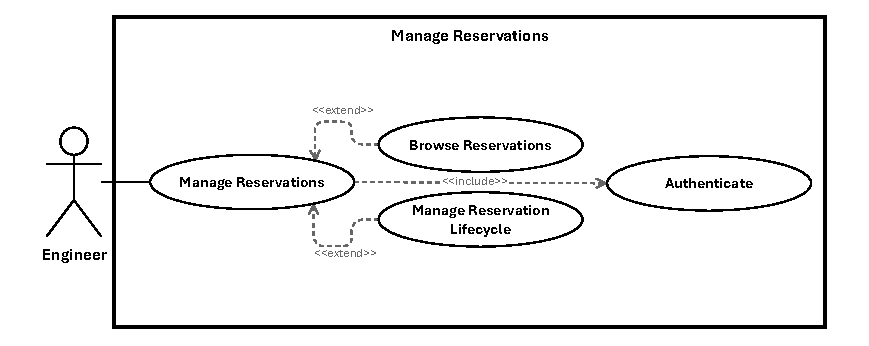
\includegraphics[width=\textwidth]{assets/chapter3/eng-manage-reservations-use-case}
    \caption{Use Case Manage Reservations}
    \label{fig:eng-manage-reservations-use-case}
\end{figure}
\dotsection{\textbf{Specification of the Use Case Browse Reservations}}
\begin{table}[H]
    \centering
    \caption{Use Case Specification: Browse Reservations}
    \begin{tabular}{|p{3.5cm}|p{10.5cm}|}
        \hline
        \textbf{Title}          & Browse Reservations \\
        \hline
        \textbf{Summary}        & Engineer views all their reservations for USB devices, cameras, and VM resources, and inspects the full details of any individual reservation \\
        \hline
        \textbf{Actor}          & Engineer \\
        \hline
        \textbf{Precondition}   & The engineer is authenticated and has created at least one reservation \\
        \hline
        \textbf{Post-condition} & Engineer has viewed their reservation list and the complete details of a selected reservation including dates, status, resource type, and any pending actions \\
        \hline
        \textbf{Basic Scenario} & \begin{minipage}[t]{\linewidth}
            \begin{enumerate}[topsep=0pt,itemsep=1pt,parsep=0pt,partopsep=0pt]
                \item Engineer navigates to the reservations section; system retrieves and displays all reservations with resource type, date range, and status; engineer may filter by resource type or status
                \item Engineer selects a reservation; system displays the full detail view showing resource type, date range, status, special requirements, approval status, and any available actions
            \end{enumerate}
        \end{minipage} \\
        \hline
        \textbf{Error Scenario} & \begin{minipage}[t]{\linewidth}
            \begin{enumerate}[topsep=0pt,itemsep=1pt,parsep=0pt,partopsep=0pt]
                \item If no reservations exist, system displays an empty state with an option to create one
                \item If a selected reservation has been deleted, system shows a not-found notice and returns to the list
            \end{enumerate}
        \end{minipage} \\
        \hline
    \end{tabular}
    \label{tab:eng-browse-reservations}
\end{table}
\dotsection{\textbf{Specification of the Use Case Manage Reservation Lifecycle}}
\begin{table}[H]
    \centering
    \caption{Use Case Specification: Manage Reservation Lifecycle}
    \begin{tabular}{|p{3.5cm}|p{10.5cm}|}
        \hline
        \textbf{Title}          & Manage Reservation Lifecycle \\
        \hline
        \textbf{Summary}        & Engineer consults the availability calendar, creates new reservations for USB devices, cameras, or VM resources, and cancels existing ones when no longer needed \\
        \hline
        \textbf{Actor}          & Engineer \\
        \hline
        \textbf{Precondition}   & The engineer is authenticated and has access to the reservation system; the desired resource must be available for new reservations \\
        \hline
        \textbf{Post-condition} & A reservation is created and pending approval, or an existing reservation is cancelled and the resource is released for other users \\
        \hline
        \textbf{Basic Scenario} & \begin{minipage}[t]{\linewidth}
            \begin{enumerate}[topsep=0pt,itemsep=1pt,parsep=0pt,partopsep=0pt]
                \item Engineer opens the reservation calendar; system displays a calendar view with resource availability and existing reservations shown as blocked time slots; engineer may navigate between dates to find a suitable slot
                \item For \textbf{Create}: engineer selects an available time slot and resource type, system checks for scheduling conflicts, engineer submits the request, system creates the reservation with pending status and confirms the submission with approval status
                \item For \textbf{Cancel}: engineer selects an existing reservation and confirms cancellation; system cancels the record, releases the resource, and makes it available for other reservations
            \end{enumerate}
        \end{minipage} \\
        \hline
        \textbf{Error Scenario} & \begin{minipage}[t]{\linewidth}
            \begin{enumerate}[topsep=0pt,itemsep=1pt,parsep=0pt,partopsep=0pt]
                \item If calendar data fails to load, system shows an error with a retry option
                \item If the selected time slot conflicts with an existing reservation, system shows alternative availability
                \item If the resource is not available, system displays availability information
                \item If the reservation has already started, cancellation may be restricted
                \item If cancellation fails, system logs the error and preserves the reservation
            \end{enumerate}
        \end{minipage} \\
        \hline
    \end{tabular}
    \label{tab:eng-reservation-lifecycle}
\end{table}

\iffalse
\dotsection{\textbf{Specification of the Use Case List USB/Cameras/VM Reservations}}
\begin{table}[H]
    \centering
    \caption{Use Case Specification: List USB/Cameras/VM Reservations}
    \begin{tabular}{|p{3.5cm}|p{10.5cm}|}
        \hline
        \textbf{Title}          & List USB/Cameras/VM Reservations                                                                 \\
        \hline
        \textbf{Summary}        & Engineer views all their reservations for USB devices, cameras, and VM resources          \\
        \hline
        \textbf{Actor}          & Engineer                                                                                       \\
        \hline
        \textbf{Precondition}   & The engineer is authenticated and has created at least one reservation                     \\
        \hline
        \textbf{Post-condition} & Engineer views a list of reservations with dates, status, and resource details            \\
        \hline
        \textbf{Basic Scenario} & \begin{minipage}[t]{\linewidth}
                                      \begin{enumerate}[topsep=0pt,itemsep=1pt,parsep=0pt,partopsep=0pt]
                                          \item Engineer navigates to the reservations section
                                          \item System retrieves all reservations for the engineer
                                          \item System displays reservations with resource type, date range, and status
                                          \item Engineer can filter by resource type or status
                                          \item Engineer can select a reservation to view details or take actions
                                      \end{enumerate}
                                  \end{minipage}  \\
        \hline
        \textbf{Error Scenario} & \begin{minipage}[t]{\linewidth}
                                      \begin{enumerate}[topsep=0pt,itemsep=1pt,parsep=0pt,partopsep=0pt]
                                          \item If no reservations exist, the system displays an empty-state with option to create one
                                      \end{enumerate}
                                  \end{minipage} \\
        \hline
    \end{tabular}
    \label{tab:eng-list-reservations}
\end{table}
\dotsection{\textbf{Specification of the Use Case View USB/Cameras/VM Reservation Details}}
\begin{table}[H]
    \centering
    \caption{Use Case Specification: View USB/Cameras/VM Reservation Details}
    \begin{tabular}{|p{3.5cm}|p{10.5cm}|}
        \hline
        \textbf{Title}          & View USB/Cameras/VM Reservation Details                                                                 \\
        \hline
        \textbf{Summary}        & Engineer views detailed information about a specific reservation                            \\
        \hline
        \textbf{Actor}          & Engineer                                                                                             \\
        \hline
        \textbf{Precondition}   & The engineer has an existing reservation                                                           \\
        \hline
        \textbf{Post-condition} & Engineer views complete reservation information including dates, status, and resource details \\
        \hline
        \textbf{Basic Scenario} & \begin{minipage}[t]{\linewidth}
                                      \begin{enumerate}[topsep=0pt,itemsep=1pt,parsep=0pt,partopsep=0pt]
                                          \item Engineer selects a reservation from their list
                                          \item System displays detailed reservation information
                                          \item System shows resource type, date range, status, and any special requirements
                                          \item System displays approval status and any pending actions
                                          \item Engineer can view or modify the reservation if allowed
                                      \end{enumerate}
                                  \end{minipage}  \\
        \hline
        \textbf{Error Scenario} & \begin{minipage}[t]{\linewidth}
                                      \begin{enumerate}[topsep=0pt,itemsep=1pt,parsep=0pt,partopsep=0pt]
                                          \item If the reservation has been deleted, the system shows a not-found notice
                                      \end{enumerate}
                                  \end{minipage} \\
        \hline
    \end{tabular}
    \label{tab:eng-view-reservation}
\end{table}
\dotsection{\textbf{Specification of the Use Case Create USB/Cameras/VM Reservation}}
\begin{table}[H]
    \centering
    \caption{Use Case Specification: Create USB/Cameras/VM Reservation}
    \begin{tabular}{|p{3.5cm}|p{10.5cm}|}
        \hline
        \textbf{Title}          & Create USB/Cameras/VM Reservation                                                                 \\
        \hline
        \textbf{Summary}        & Engineer creates a new reservation for USB devices, cameras, or VM resources              \\
        \hline
        \textbf{Actor}          & Engineer                                                                                         \\
        \hline
        \textbf{Precondition}   & The engineer is authenticated and the desired resource is available for reservation        \\
        \hline
        \textbf{Post-condition} & A reservation is created and awaits approval according to the reservation policy            \\
        \hline
        \textbf{Basic Scenario} & \begin{minipage}[t]{\linewidth}
                                      \begin{enumerate}[topsep=0pt,itemsep=1pt,parsep=0pt,partopsep=0pt]
                                          \item Engineer navigates to the reservation creation interface
                                          \item System displays available resources and calendar
                                          \item Engineer selects resource type and desired time range
                                          \item System checks for conflicts with existing reservations
                                          \item Engineer submits the reservation request
                                          \item System creates the reservation with pending status
                                          \item System confirms the reservation and displays approval status
                                      \end{enumerate}
                                  \end{minipage}  \\
        \hline
        \textbf{Error Scenario} & \begin{minipage}[t]{\linewidth}
                                      \begin{enumerate}[topsep=0pt,itemsep=1pt,parsep=0pt,partopsep=0pt]
                                          \item If the time slot conflicts with an existing reservation, the system shows alternatives
                                          \item If the resource is not available, the system displays availability information
                                      \end{enumerate}
                                  \end{minipage} \\
        \hline
    \end{tabular}
    \label{tab:eng-create-reservation}
\end{table}
\dotsection{\textbf{Specification of the Use Case View USB/Cameras/VM Reservation Calendar}}
\begin{table}[H]
    \centering
    \caption{Use Case Specification: View USB/Cameras/VM Reservation Calendar}
    \begin{tabular}{|p{3.5cm}|p{10.5cm}|}
        \hline
        \textbf{Title}          & View USB/Cameras/VM Reservation Calendar                                                                 \\
        \hline
        \textbf{Summary}        & Engineer views a calendar showing availability and existing reservations for resources    \\
        \hline
        \textbf{Actor}          & Engineer                                                                                              \\
        \hline
        \textbf{Precondition}   & The engineer is authenticated and has access to the reservation system                     \\
        \hline
        \textbf{Post-condition} & Engineer views a calendar with resource availability and reservation information        \\
        \hline
        \textbf{Basic Scenario} & \begin{minipage}[t]{\linewidth}
                                      \begin{enumerate}[topsep=0pt,itemsep=1pt,parsep=0pt,partopsep=0pt]
                                          \item Engineer navigates to the reservation calendar
                                          \item System displays a calendar view with resource availability
                                          \item System shows existing reservations as blocked time slots
                                          \item Engineer can navigate between dates and view availability
                                          \item Engineer can select available time slots to create new reservations
                                      \end{enumerate}
                                  \end{minipage}  \\
        \hline
        \textbf{Error Scenario} & \begin{minipage}[t]{\linewidth}
                                      \begin{enumerate}[topsep=0pt,itemsep=1pt,parsep=0pt,partopsep=0pt]
                                          \item If calendar data fails to load, the system shows an error with retry option
                                      \end{enumerate}
                                  \end{minipage} \\
        \hline
    \end{tabular}
    \label{tab:eng-reservation-calendar}
\end{table}
\dotsection{\textbf{Specification of the Use Case Cancel USB/Cameras/VM Reservation}}
\begin{table}[H]
    \centering
    \caption{Use Case Specification: Cancel USB/Cameras/VM Reservation}
    \begin{tabular}{|p{3.5cm}|p{10.5cm}|}
        \hline
        \textbf{Title}          & Cancel USB/Cameras/VM Reservation                                                                 \\
        \hline
        \textbf{Summary}        & Engineer cancels an existing reservation for USB devices, cameras, or VM resources        \\
        \hline
        \textbf{Actor}          & Engineer                                                                                          \\
        \hline
        \textbf{Precondition}   & The engineer has an existing reservation that can be cancelled                                 \\
        \hline
        \textbf{Post-condition} & The reservation is cancelled and the resource is made available to other users                \\
        \hline
        \textbf{Basic Scenario} & \begin{minipage}[t]{\linewidth}
                                      \begin{enumerate}[topsep=0pt,itemsep=1pt,parsep=0pt,partopsep=0pt]
                                          \item Engineer views their reservations
                                          \item Engineer selects a reservation to cancel
                                          \item System displays cancellation confirmation
                                          \item Engineer confirms the cancellation
                                          \item System cancels the reservation and updates status
                                          \item Resource is released and available for other reservations
                                      \end{enumerate}
                                  \end{minipage}  \\
        \hline
        \textbf{Error Scenario} & \begin{minipage}[t]{\linewidth}
                                      \begin{enumerate}[topsep=0pt,itemsep=1pt,parsep=0pt,partopsep=0pt]
                                          \item If the reservation has already started, cancellation may be restricted
                                          \item If cancellation fails, the system logs the error and preserves the reservation
                                      \end{enumerate}
                                  \end{minipage} \\
        \hline
    \end{tabular}
    \label{tab:eng-cancel-reservation}
\end{table}
\fi

\subsubsubsection[Manage Virtual Lab]{Refinement of the Use Case Manage Virtual Lab} Figure
\ref{fig:eng-manage-virtual-lab-use-case} presents the refinement of the
Use Case Manage Virtual Lab for the Engineer actor. This use case includes
the following sub-use cases:
\begin{figure}[H]
    \centering
    
\includegraphics[width=\textwidth]{assets/chapter3/eng-manage-virtual-lab-use-case}
    \caption{Use Case Manage Virtual Lab}
    \label{fig:eng-manage-virtual-lab-use-case}
\end{figure}
\dotsection{\textbf{Specification of the Use Case Manage VM Sessions}}
\begin{table}[H]
    \centering
    \caption{Use Case Specification: Manage VM Sessions}
    \begin{tabular}{|p{3.5cm}|p{10.5cm}|}
        \hline
        \textbf{Title}          & Manage VM Sessions \\
        \hline
        \textbf{Summary}        & Engineer views, provisions, extends, and terminates virtual machine sessions to access and manage their remote laboratory environment \\
        \hline
        \textbf{Actor}          & Engineer (and Administrator when authorized) \\
        \hline
        \textbf{Precondition}   & The engineer is authenticated, verified, and authorized through the \texttt{provision-vm} ability where applicable \\
        \hline
        \textbf{Post-condition} & The VM session is created, extended, or terminated and infrastructure resources are allocated or released accordingly \\
        \hline
        \textbf{Basic Scenario} & \begin{minipage}[t]{\linewidth}
            \begin{enumerate}[topsep=0pt,itemsep=1pt,parsep=0pt,partopsep=0pt]
                \item Engineer opens the VM sessions interface; system displays all sessions with status (active, expired, terminated), creation time, and remaining duration; engineer may filter by status or date range
                \item For \textbf{Provision}: engineer submits a request to create a new session; system validates authorization and rate-limit constraints, selects suitable server and node resources, provisions the session record with associated infrastructure metadata, and returns the created session to the interface
                \item For \textbf{Extend}: engineer selects an active session and chooses an extension duration; system validates eligibility and rate limits, updates the expiration time, and confirms the new deadline
                \item For \textbf{Terminate}: engineer confirms the termination of an active session; system validates the request, releases associated infrastructure resources, and marks the session as terminated
            \end{enumerate}
        \end{minipage} \\
        \hline
        \textbf{Error Scenario} & \begin{minipage}[t]{\linewidth}
            \begin{enumerate}[topsep=0pt,itemsep=1pt,parsep=0pt,partopsep=0pt]
                \item If no sessions exist, system displays an empty state with an option to provision one
                \item Authorization failure or rate-limit excess prevents provisioning and surfaces an explanatory error
                \item If no infrastructure capacity is available, system returns a controlled failure
                \item Extension is blocked if the session has expired or the maximum extension limit is reached
                \item If termination fails, system logs the error and preserves the session state
                \item Provisioning or extension failures preserve traceability through logs or alerts
            \end{enumerate}
        \end{minipage} \\
        \hline
    \end{tabular}
    \label{tab:eng-manage-sessions}
\end{table}
\dotsection{\textbf{Specification of the Use Case Manage Session Devices}}
\begin{table}[H]
    \centering
    \caption{Use Case Specification: Manage Session Devices}
    \begin{tabular}{|p{3.5cm}|p{10.5cm}|}
        \hline
        \textbf{Title}          & Manage Session Devices \\
        \hline
        \textbf{Summary}        & Engineer attaches and detaches USB devices to and from an active VM session, and joins a waiting queue when a desired device is currently in use \\
        \hline
        \textbf{Actor}          & Engineer \\
        \hline
        \textbf{Precondition}   & The engineer has an active VM session \\
        \hline
        \textbf{Post-condition} & The device is attached to or detached from the session, or the engineer is queued and notified when the device becomes available \\
        \hline
        \textbf{Basic Scenario} & \begin{minipage}[t]{\linewidth}
            \begin{enumerate}[topsep=0pt,itemsep=1pt,parsep=0pt,partopsep=0pt]
                \item Engineer views their active session; system displays available devices with availability status
                \item For \textbf{Attach}: engineer selects an available device; system validates compatibility and availability, establishes the connection between the device and the VM, and confirms attachment; the device becomes accessible from within the VM environment
                \item For \textbf{Detach}: engineer selects an attached device and confirms detachment; system disconnects the device, releases it for use by other sessions, and confirms the action
                \item For \textbf{Queue}: if the desired device is in use, engineer selects the option to join the waiting queue; system adds the engineer with their queue position and estimated wait time, and notifies them when the device becomes available
            \end{enumerate}
        \end{minipage} \\
        \hline
        \textbf{Error Scenario} & \begin{minipage}[t]{\linewidth}
            \begin{enumerate}[topsep=0pt,itemsep=1pt,parsep=0pt,partopsep=0pt]
                \item If the device is already in use, system displays availability information and offers the queue option
                \item If the device is incompatible with the VM, system prevents attachment
                \item If attachment or detachment fails, system logs the error and allows retry
                \item If detachment is requested while a process is actively using the device, system warns or delays the action
                \item If the engineer is already in the queue, system displays their current position
                \item If the queue is full, system prevents joining and displays capacity information
            \end{enumerate}
        \end{minipage} \\
        \hline
    \end{tabular}
    \label{tab:eng-manage-devices}
\end{table}
\dotsection{\textbf{Specification of the Use Case Access Laboratory Cameras}}
\begin{table}[H]
    \centering
    \caption{Use Case Specification: Access Laboratory Cameras}
    \begin{tabular}{|p{3.5cm}|p{10.5cm}|}
        \hline
        \textbf{Title}          & Access Laboratory Cameras \\
        \hline
        \textbf{Summary}        & Engineer browses available laboratory cameras, views their live streams, and adjusts stream resolution to monitor laboratory equipment during an active VM session \\
        \hline
        \textbf{Actor}          & Engineer \\
        \hline
        \textbf{Precondition}   & The engineer has an active VM session and at least one camera is configured for the laboratory \\
        \hline
        \textbf{Post-condition} & Engineer is viewing a live camera stream at the selected resolution \\
        \hline
        \textbf{Basic Scenario} & \begin{minipage}[t]{\linewidth}
            \begin{enumerate}[topsep=0pt,itemsep=1pt,parsep=0pt,partopsep=0pt]
                \item Engineer opens the camera panel for their active session; system displays available cameras with status (available, in use, offline) and capabilities (PTZ support, resolution options)
                \item Engineer selects a camera; system displays available resolution options with details (width, height, frame rate, bandwidth requirements)
                \item Engineer selects a resolution; system initiates the stream connection and displays the live video feed in a player window
                \item Engineer may switch resolution at any time while viewing; system reconfigures the stream and updates bandwidth requirements accordingly
                \item Stream continues until the engineer stops viewing or the session ends
            \end{enumerate}
        \end{minipage} \\
        \hline
        \textbf{Error Scenario} & \begin{minipage}[t]{\linewidth}
            \begin{enumerate}[topsep=0pt,itemsep=1pt,parsep=0pt,partopsep=0pt]
                \item If no cameras are available or configured, system displays an empty state
                \item If camera status cannot be retrieved, system shows an error with a retry option
                \item If a camera is offline, system displays an unavailable message
                \item If the stream fails to load, system offers retry and may suggest a lower resolution
                \item If resolution switching fails, system preserves the current resolution
            \end{enumerate}
        \end{minipage} \\
        \hline
    \end{tabular}
    \label{tab:eng-access-cameras}
\end{table}
\dotsection{\textbf{Specification of the Use Case Control PTZ Camera}}
\begin{table}[H]
    \centering
    \caption{Use Case Specification: Control PTZ Camera}
    \begin{tabular}{|p{3.5cm}|p{10.5cm}|}
        \hline
        \textbf{Title}          & Control PTZ Camera \\
        \hline
        \textbf{Summary}        & Engineer acquires exclusive control over a PTZ camera, sends pan, tilt, and zoom commands to adjust its view, and releases control when finished \\
        \hline
        \textbf{Actor}          & Engineer \\
        \hline
        \textbf{Precondition}   & The engineer has an active VM session and is viewing a camera that supports PTZ control \\
        \hline
        \textbf{Post-condition} & Camera control is acquired, commands are applied, and control is released and made available to other users \\
        \hline
        \textbf{Basic Scenario} & \begin{minipage}[t]{\linewidth}
            \begin{enumerate}[topsep=0pt,itemsep=1pt,parsep=0pt,partopsep=0pt]
                \item Engineer views a PTZ-capable camera stream; system displays control availability status
                \item Engineer requests camera control; system checks availability and if free grants exclusive control to the engineer, updates control status, and notifies other users
                \item Engineer uses the PTZ control interface to send pan (horizontal), tilt (vertical), and zoom commands; system forwards each command to the camera, which moves to the new position; stream updates to reflect the new view
                \item When finished, engineer releases control; system revokes exclusive access, marks the camera as available, and notifies other users
            \end{enumerate}
        \end{minipage} \\
        \hline
        \textbf{Error Scenario} & \begin{minipage}[t]{\linewidth}
            \begin{enumerate}[topsep=0pt,itemsep=1pt,parsep=0pt,partopsep=0pt]
                \item If the camera does not support PTZ, system disables control options
                \item If the camera is already controlled by another user, system displays a queue option
                \item If a PTZ command is out of range or invalid, system ignores or limits it
                \item If the camera does not respond to a command, system displays an error
                \item If control release fails, system logs the error and preserves the current control state
            \end{enumerate}
        \end{minipage} \\
        \hline
    \end{tabular}
    \label{tab:eng-ptz-control}
\end{table}

\iffalse
\dotsection{\textbf{Specification of the Use Case List My VM Sessions}}
\begin{table}[H]
    \centering
    \caption{Use Case Specification: List My VM Sessions}
    \begin{tabular}{|p{3.5cm}|p{10.5cm}|}
        \hline
        \textbf{Title}          & List My VM Sessions                                                                 \\
        \hline
        \textbf{Summary}        & Engineer views all their virtual machine sessions including active and historical ones \\
        \hline
        \textbf{Actor}          & Engineer                                                                             \\
        \hline
        \textbf{Precondition}   & The engineer is authenticated and has created at least one VM session                 \\
        \hline
        \textbf{Post-condition} & Engineer views a list of VM sessions with status, duration, and resource details     \\
        \hline
        \textbf{Basic Scenario} & \begin{minipage}[t]{\linewidth}
                                      \begin{enumerate}[topsep=0pt,itemsep=1pt,parsep=0pt,partopsep=0pt]
                                          \item Engineer navigates to the VM sessions section
                                          \item System retrieves all VM sessions for the engineer
                                          \item System displays sessions with status (active, expired, terminated), creation time,
                                                and remaining duration
                                          \item Engineer can filter by status or date range
                                          \item Engineer can select a session to view details or take actions
                                      \end{enumerate}
                                  \end{minipage}  \\
        \hline
        \textbf{Error Scenario} & \begin{minipage}[t]{\linewidth}
                                      \begin{enumerate}[topsep=0pt,itemsep=1pt,parsep=0pt,partopsep=0pt]
                                          \item If no sessions exist, the system displays an empty-state with option to create one
                                      \end{enumerate}
                                  \end{minipage} \\
        \hline
    \end{tabular}
    \label{tab:eng-list-sessions}
\end{table}
\dotsection{\textbf{Specification of the Use Case Provision (Create) VM Session}}
\begin{table}[H]
    \centering
    \caption{Use Case Specification: Provision (Create) VM Session}
    \begin{tabular}{|p{3.5cm}|p{10.5cm}|}
        \hline
        \textbf{Title}          & Provision (Create) VM Session                                                                                       \\
        \hline
        \textbf{Summary}        & Engineer creates a time-bound virtual machine session in order to access a remote laboratory environment                \\
        \hline
        \textbf{Actor}          & Engineer (and Administrator when authorized)                                                                            \\
        \hline
        \textbf{Precondition}   & User is authenticated, verified, and authorized through the \texttt{provision-vm} ability                               \\
        \hline
        \textbf{Post-condition} & A VM session is created, linked to a compute node and server context, and made available for later access and extension \\
        \hline
        \textbf{Basic Scenario} &
        \begin{minipage}[t]{\linewidth}
            \begin{enumerate}[topsep=0pt,itemsep=1pt,parsep=0pt,partopsep=0pt]
                \item Engineer opens the sessions interface
                \item System displays active or previous sessions
                \item Engineer submits a request to create a new session
                \item System validates authorization and rate-limit constraints
                \item System selects suitable server and node resources
                \item System provisions a session record and associates infrastructure metadata
                \item System returns the created session to the user interface
                \item Engineer can subsequently view, extend, or terminate the session
            \end{enumerate}
        \end{minipage}                                                            \\
        \hline
        \textbf{Error Scenario} &
        \begin{minipage}[t]{\linewidth}
            \begin{enumerate}[topsep=0pt,itemsep=1pt,parsep=0pt,partopsep=0pt]
                \item If authorization fails, the system rejects the request
                \item If rate limits are exceeded, the system delays the operation
                \item If no infrastructure capacity is available, the system returns a controlled
                      failure
                \item If provisioning fails, the system preserves traceability through logs or alerts
            \end{enumerate}
        \end{minipage}                                                      \\
        \hline
    \end{tabular}
    \label{tab:eng-provision-session}
\end{table}
\dotsection{\textbf{Specification of the Use Case Extend Session Duration}}
\begin{table}[H]
    \centering
    \caption{Use Case Specification: Extend Session Duration}
    \begin{tabular}{|p{3.5cm}|p{10.5cm}|}
        \hline
        \textbf{Title}          & Extend Session Duration                                                                 \\
        \hline
        \textbf{Summary}        & Engineer extends the duration of an active VM session to continue laboratory work        \\
        \hline
        \textbf{Actor}          & Engineer                                                                                \\
        \hline
        \textbf{Precondition}   & The engineer has an active VM session that has not reached maximum extension limits   \\
        \hline
        \textbf{Post-condition} & The session duration is extended and the new expiration time is updated                 \\
        \hline
        \textbf{Basic Scenario} & \begin{minipage}[t]{\linewidth}
                                      \begin{enumerate}[topsep=0pt,itemsep=1pt,parsep=0pt,partopsep=0pt]
                                          \item Engineer views their active VM session
                                          \item System displays remaining time and extension options
                                          \item Engineer selects an extension duration
                                          \item System validates extension eligibility and rate limits
                                          \item System updates the session expiration time
                                          \item System confirms the extension and displays new expiration
                                      \end{enumerate}
                                  \end{minipage}  \\
        \hline
        \textbf{Error Scenario} & \begin{minipage}[t]{\linewidth}
                                      \begin{enumerate}[topsep=0pt,itemsep=1pt,parsep=0pt,partopsep=0pt]
                                          \item If the session has expired, extension is not allowed
                                          \item If maximum extension limit is reached, the system displays the restriction
                                          \item If rate limits are exceeded, the system delays the operation
                                      \end{enumerate}
                                  \end{minipage} \\
        \hline
    \end{tabular}
    \label{tab:eng-extend-session}
\end{table}
\dotsection{\textbf{Specification of the Use Case Terminate Session}}
\begin{table}[H]
    \centering
    \caption{Use Case Specification: Terminate Session}
    \begin{tabular}{|p{3.5cm}|p{10.5cm}|}
        \hline
        \textbf{Title}          & Terminate Session                                                                 \\
        \hline
        \textbf{Summary}        & Engineer terminates an active VM session to release resources and end laboratory work \\
        \hline
        \textbf{Actor}          & Engineer                                                                           \\
        \hline
        \textbf{Precondition}   & The engineer has an active VM session                                              \\
        \hline
        \textbf{Post-condition} & The session is terminated, resources are released, and the session is marked as ended \\
        \hline
        \textbf{Basic Scenario} & \begin{minipage}[t]{\linewidth}
                                      \begin{enumerate}[topsep=0pt,itemsep=1pt,parsep=0pt,partopsep=0pt]
                                          \item Engineer views their active VM session
                                          \item System displays termination option
                                          \item Engineer confirms termination
                                          \item System validates the termination request
                                          \item System terminates the session and releases associated resources
                                          \item System updates session status to terminated
                                          \item Engineer can no longer access the VM through this session
                                      \end{enumerate}
                                  \end{minipage}  \\
        \hline
        \textbf{Error Scenario} & \begin{minipage}[t]{\linewidth}
                                      \begin{enumerate}[topsep=0pt,itemsep=1pt,parsep=0pt,partopsep=0pt]
                                          \item If the session is already terminated, the system displays the current status
                                          \item If termination fails, the system logs the error and preserves the session state
                                      \end{enumerate}
                                  \end{minipage} \\
        \hline
    \end{tabular}
    \label{tab:eng-terminate-session}
\end{table}
\dotsection{\textbf{Specification of the Use Case Attach Device to Session}}
\begin{table}[H]
    \centering
    \caption{Use Case Specification: Attach Device to Session}
    \begin{tabular}{|p{3.5cm}|p{10.5cm}|}
        \hline
        \textbf{Title}          & Attach Device to Session                                                                 \\
        \hline
        \textbf{Summary}        & Engineer attaches a USB device or camera to their active VM session for laboratory work \\
        \hline
        \textbf{Actor}          & Engineer                                                                                 \\
        \hline
        \textbf{Precondition}   & The engineer has an active VM session and the device is available and not in use        \\
        \hline
        \textbf{Post-condition} & The device is attached to the session and accessible from within the VM                 \\
        \hline
        \textbf{Basic Scenario} & \begin{minipage}[t]{\linewidth}
                                      \begin{enumerate}[topsep=0pt,itemsep=1pt,parsep=0pt,partopsep=0pt]
                                          \item Engineer views their active VM session
                                          \item System displays available devices for attachment
                                          \item Engineer selects a device to attach
                                          \item System validates device availability and session compatibility
                                          \item System establishes the connection between device and VM
                                          \item System confirms attachment and displays device status
                                          \item Device is now accessible from within the VM environment
                                      \end{enumerate}
                                  \end{minipage}  \\
        \hline
        \textbf{Error Scenario} & \begin{minipage}[t]{\linewidth}
                                      \begin{enumerate}[topsep=0pt,itemsep=1pt,parsep=0pt,partopsep=0pt]
                                          \item If the device is already in use, the system displays availability information
                                          \item If the device is not compatible with the VM, the system prevents attachment
                                          \item If attachment fails, the system logs the error and allows retry
                                      \end{enumerate}
                                  \end{minipage} \\
        \hline
    \end{tabular}
    \label{tab:eng-attach-device}
\end{table}
\dotsection{\textbf{Specification of the Use Case Detach Device from Session}}
\begin{table}[H]
    \centering
    \caption{Use Case Specification: Detach Device from Session}
    \begin{tabular}{|p{3.5cm}|p{10.5cm}|}
        \hline
        \textbf{Title}          & Detach Device from Session                                                                 \\
        \hline
        \textbf{Summary}        & Engineer detaches a USB device or camera from their active VM session                     \\
        \hline
        \textbf{Actor}          & Engineer                                                                                   \\
        \hline
        \textbf{Precondition}   & The engineer has an active VM session with an attached device                            \\
        \hline
        \textbf{Post-condition} & The device is detached from the session and released for use by other sessions         \\
        \hline
        \textbf{Basic Scenario} & \begin{minipage}[t]{\linewidth}
                                      \begin{enumerate}[topsep=0pt,itemsep=1pt,parsep=0pt,partopsep=0pt]
                                          \item Engineer views their active VM session
                                          \item System displays currently attached devices
                                          \item Engineer selects a device to detach
                                          \item System validates the detachment request
                                          \item System disconnects the device from the VM
                                          \item System confirms detachment and releases the device
                                          \item Device is no longer accessible from the VM
                                      \end{enumerate}
                                  \end{minipage}  \\
        \hline
        \textbf{Error Scenario} & \begin{minipage}[t]{\linewidth}
                                      \begin{enumerate}[topsep=0pt,itemsep=1pt,parsep=0pt,partopsep=0pt]
                                          \item If the device is in use by an active process, the system may warn or delay detachment
                                          \item If detachment fails, the system logs the error and preserves the connection
                                      \end{enumerate}
                                  \end{minipage} \\
        \hline
    \end{tabular}
    \label{tab:eng-detach-device}
\end{table}
\dotsection{\textbf{Specification of the Use Case Join Device Queue}}
\begin{table}[H]
    \centering
    \caption{Use Case Specification: Join Device Queue}
    \begin{tabular}{|p{3.5cm}|p{10.5cm}|}
        \hline
        \textbf{Title}          & Join Device Queue                                                                 \\
        \hline
        \textbf{Summary}        & Engineer joins a waiting queue for a device that is currently in use by another session \\
        \hline
        \textbf{Actor}          & Engineer                                                                           \\
        \hline
        \textbf{Precondition}   & The engineer has an active VM session and the desired device is currently unavailable \\
        \hline
        \textbf{Post-condition} & The engineer is added to the device queue and will be notified when the device becomes available \\
        \hline
        \textbf{Basic Scenario} & \begin{minipage}[t]{\linewidth}
                                      \begin{enumerate}[topsep=0pt,itemsep=1pt,parsep=0pt,partopsep=0pt]
                                          \item Engineer views available devices for their session
                                          \item System indicates that a device is currently in use
                                          \item Engineer selects the option to join the waiting queue
                                          \item System adds the engineer to the queue with their position
                                          \item System displays estimated wait time and queue position
                                          \item When the device becomes available, the system notifies the engineer
                                          \item Engineer can then attach the device to their session
                                      \end{enumerate}
                                  \end{minipage}  \\
        \hline
        \textbf{Error Scenario} & \begin{minipage}[t]{\linewidth}
                                      \begin{enumerate}[topsep=0pt,itemsep=1pt,parsep=0pt,partopsep=0pt]
                                          \item If the engineer is already in the queue, the system displays their current position
                                          \item If the queue is full, the system prevents joining and displays capacity information
                                      \end{enumerate}
                                  \end{minipage} \\
        \hline
    \end{tabular}
    \label{tab:eng-join-queue}
\end{table}
\dotsection{\textbf{Specification of the Use Case List Cameras for Session}}
\begin{table}[H]
    \centering
    \caption{Use Case Specification: List Cameras for Session}
    \begin{tabular}{|p{3.5cm}|p{10.5cm}|}
        \hline
        \textbf{Title}          & List Cameras for Session                                                                 \\
        \hline
        \textbf{Summary}        & Engineer views available cameras that can be accessed for their active VM session       \\
        \hline
        \textbf{Actor}          & Engineer                                                                                  \\
        \hline
        \textbf{Precondition}   & The engineer has an active VM session and cameras are configured for the laboratory     \\
        \hline
        \textbf{Post-condition} & Engineer views a list of available cameras with their status and capabilities           \\
        \hline
        \textbf{Basic Scenario} & \begin{minipage}[t]{\linewidth}
                                      \begin{enumerate}[topsep=0pt,itemsep=1pt,parsep=0pt,partopsep=0pt]
                                          \item Engineer views their active VM session
                                          \item System displays available cameras for the session
                                          \item System shows camera status (available, in use, offline)
                                          \item System displays camera capabilities (PTZ support, resolution options)
                                          \item Engineer can select a camera to view its stream or control it
                                      \end{enumerate}
                                  \end{minipage}  \\
        \hline
        \textbf{Error Scenario} & \begin{minipage}[t]{\linewidth}
                                      \begin{enumerate}[topsep=0pt,itemsep=1pt,parsep=0pt,partopsep=0pt]
                                          \item If no cameras are available, the system displays an empty-state message
                                          \item If camera status cannot be retrieved, the system shows an error with retry option
                                      \end{enumerate}
                                  \end{minipage} \\
        \hline
    \end{tabular}
    \label{tab:eng-list-cameras}
\end{table}
\dotsection{\textbf{Specification of the Use Case View Camera Resolutions}}
\begin{table}[H]
    \centering
    \caption{Use Case Specification: View Camera Resolutions}
    \begin{tabular}{|p{3.5cm}|p{10.5cm}|}
        \hline
        \textbf{Title}          & View Camera Resolutions                                                                 \\
        \hline
        \textbf{Summary}        & Engineer views available resolution options for a selected camera stream                \\
        \hline
        \textbf{Actor}          & Engineer                                                                                \\
        \hline
        \textbf{Precondition}   & The engineer has selected a camera that supports multiple resolution options            \\
        \hline
        \textbf{Post-condition} & Engineer views available resolutions and can select the desired quality                  \\
        \hline
        \textbf{Basic Scenario} & \begin{minipage}[t]{\linewidth}
                                      \begin{enumerate}[topsep=0pt,itemsep=1pt,parsep=0pt,partopsep=0pt]
                                          \item Engineer selects a camera from the available list
                                          \item System displays the camera's available resolution options
                                          \item System shows resolution details (width, height, frame rate, bandwidth requirements)
                                          \item Engineer can select a resolution for the stream
                                          \item System applies the selected resolution to the camera stream
                                      \end{enumerate}
                                  \end{minipage}  \\
        \hline
        \textbf{Error Scenario} & \begin{minipage}[t]{\linewidth}
                                      \begin{enumerate}[topsep=0pt,itemsep=1pt,parsep=0pt,partopsep=0pt]
                                          \item If the camera does not support multiple resolutions, the system shows the default
                                          \item If resolution switching fails, the system preserves the current resolution
                                      \end{enumerate}
                                  \end{minipage} \\
        \hline
    \end{tabular}
    \label{tab:eng-camera-resolutions}
\end{table}
\dotsection{\textbf{Specification of the Use Case View Camera Stream}}
\begin{table}[H]
    \centering
    \caption{Use Case Specification: View Camera Stream}
    \begin{tabular}{|p{3.5cm}|p{10.5cm}|}
        \hline
        \textbf{Title}          & View Camera Stream                                                                 \\
        \hline
        \textbf{Summary}        & Engineer views the live video stream from a laboratory camera                          \\
        \hline
        \textbf{Actor}          & Engineer                                                                            \\
        \hline
        \textbf{Precondition}   & The engineer has an active VM session and the camera is available and online         \\
        \hline
        \textbf{Post-condition} & Engineer views the live camera stream in the browser or application                  \\
        \hline
        \textbf{Basic Scenario} & \begin{minipage}[t]{\linewidth}
                                      \begin{enumerate}[topsep=0pt,itemsep=1pt,parsep=0pt,partopsep=0pt]
                                          \item Engineer selects a camera from the available list
                                          \item System initiates the camera stream connection
                                          \item System displays the live video feed in a player window
                                          \item Engineer can view the stream to monitor laboratory equipment
                                          \item Stream continues until the engineer stops viewing or the session ends
                                      \end{enumerate}
                                  \end{minipage}  \\
        \hline
        \textbf{Error Scenario} & \begin{minipage}[t]{\linewidth}
                                      \begin{enumerate}[topsep=0pt,itemsep=1pt,parsep=0pt,partopsep=0pt]
                                          \item If the camera is offline, the system displays an error message
                                          \item If the stream fails to load, the system offers retry options
                                          \item If bandwidth is insufficient, the system may suggest lower resolution
                                      \end{enumerate}
                                  \end{minipage} \\
        \hline
    \end{tabular}
    \label{tab:eng-camera-stream}
\end{table}
\dotsection{\textbf{Specification of the Use Case Acquire Camera Control}}
\begin{table}[H]
    \centering
    \caption{Use Case Specification: Acquire Camera Control}
    \begin{tabular}{|p{3.5cm}|p{10.5cm}|}
        \hline
        \textbf{Title}          & Acquire Camera Control                                                                 \\
        \hline
        \textbf{Summary}        & Engineer requests exclusive control over a PTZ camera to move and adjust its view      \\
        \hline
        \textbf{Actor}          & Engineer                                                                                \\
        \hline
        \textbf{Precondition}   & The engineer has an active VM session and the camera supports PTZ control              \\
        \hline
        \textbf{Post-condition} & Engineer gains exclusive control over the camera and can send PTZ commands             \\
        \hline
        \textbf{Basic Scenario} & \begin{minipage}[t]{\linewidth}
                                      \begin{enumerate}[topsep=0pt,itemsep=1pt,parsep=0pt,partopsep=0pt]
                                          \item Engineer views a camera stream
                                          \item System displays control status and availability
                                          \item Engineer requests camera control
                                          \item System checks if camera is available for control
                                          \item If available, system grants exclusive control to the engineer
                                          \item System updates control status and notifies other users
                                          \item Engineer can now send PTZ commands to move the camera
                                      \end{enumerate}
                                  \end{minipage}  \\
        \hline
        \textbf{Error Scenario} & \begin{minipage}[t]{\linewidth}
                                      \begin{enumerate}[topsep=0pt,itemsep=1pt,parsep=0pt,partopsep=0pt]
                                          \item If the camera is already controlled by another user, the system shows queue option
                                          \item If the camera does not support PTZ, the system disables control options
                                      \end{enumerate}
                                  \end{minipage} \\
        \hline
    \end{tabular}
    \label{tab:eng-acquire-camera}
\end{table}
\dotsection{\textbf{Specification of the Use Case Release Camera Control}}
\begin{table}[H]
    \centering
    \caption{Use Case Specification: Release Camera Control}
    \begin{tabular}{|p{3.5cm}|p{10.5cm}|}
        \hline
        \textbf{Title}          & Release Camera Control                                                                 \\
        \hline
        \textbf{Summary}        & Engineer releases exclusive control over a PTZ camera, making it available to others     \\
        \hline
        \textbf{Actor}          & Engineer                                                                                \\
        \hline
        \textbf{Precondition}   & The engineer currently has exclusive control over the camera                            \\
        \hline
        \textbf{Post-condition} & Camera control is released and other users can request control                         \\
        \hline
        \textbf{Basic Scenario} & \begin{minipage}[t]{\linewidth}
                                      \begin{enumerate}[topsep=0pt,itemsep=1pt,parsep=0pt,partopsep=0pt]
                                          \item Engineer has control over a PTZ camera
                                          \item System displays release control option
                                          \item Engineer clicks to release camera control
                                          \item System revokes exclusive control from the engineer
                                          \item System updates camera status to available
                                          \item System notifies other users that control is available
                                          \item Camera can now be controlled by another user
                                      \end{enumerate}
                                  \end{minipage}  \\
        \hline
        \textbf{Error Scenario} & \begin{minipage}[t]{\linewidth}
                                      \begin{enumerate}[topsep=0pt,itemsep=1pt,parsep=0pt,partopsep=0pt]
                                          \item If control release fails, the system logs the error and preserves current state
                                      \end{enumerate}
                                  \end{minipage} \\
        \hline
    \end{tabular}
    \label{tab:eng-release-camera}
\end{table}
\dotsection{\textbf{Specification of the Use Case Send PTZ Move Command}}
\begin{table}[H]
    \centering
    \caption{Use Case Specification: Send PTZ Move Command}
    \begin{tabular}{|p{3.5cm}|p{10.5cm}|}
        \hline
        \textbf{Title}          & Send PTZ Move Command                                                                 \\
        \hline
        \textbf{Summary}        & Engineer controls a PTZ camera by sending pan, tilt, and zoom commands                 \\
        \hline
        \textbf{Actor}          & Engineer                                                                              \\
        \hline
        \textbf{Precondition}   & The engineer has exclusive control over a PTZ camera                                  \\
        \hline
        \textbf{Post-condition} & The camera moves to the specified position and zoom level                              \\
        \hline
        \textbf{Basic Scenario} & \begin{minipage}[t]{\linewidth}
                                      \begin{enumerate}[topsep=0pt,itemsep=1pt,parsep=0pt,partopsep=0pt]
                                          \item Engineer has control over a PTZ camera
                                          \item System displays PTZ control interface
                                          \item Engineer adjusts pan (horizontal), tilt (vertical), or zoom controls
                                          \item System sends the PTZ command to the camera
                                          \item Camera moves to the new position and zoom level
                                          \item System updates the camera stream to reflect the new view
                                      \end{enumerate}
                                  \end{minipage}  \\
        \hline
        \textbf{Error Scenario} & \begin{minipage}[t]{\linewidth}
                                      \begin{enumerate}[topsep=0pt,itemsep=1pt,parsep=0pt,partopsep=0pt]
                                          \item If the command is invalid or out of range, the system ignores or limits it
                                          \item if the camera does not respond, the system displays an error
                                      \end{enumerate}
                                  \end{minipage} \\
        \hline
    \end{tabular}
    \label{tab:eng-ptz-move}
\end{table}
\dotsection{\textbf{Specification of the Use Case Set Stream Resolution}}
\begin{table}[H]
    \centering
    \caption{Use Case Specification: Set Stream Resolution}
    \begin{tabular}{|p{3.5cm}|p{10.5cm}|}
        \hline
        \textbf{Title}          & Set Stream Resolution                                                                 \\
        \hline
        \textbf{Summary}        & Engineer changes the resolution of a camera stream to optimize quality or bandwidth    \\
        \hline
        \textbf{Actor}          & Engineer                                                                              \\
        \hline
        \textbf{Precondition}   & The engineer is viewing a camera stream that supports multiple resolutions            \\
        \hline
        \textbf{Post-condition} & The camera stream is updated to the selected resolution                                \\
        \hline
        \textbf{Basic Scenario} & \begin{minipage}[t]{\linewidth}
                                      \begin{enumerate}[topsep=0pt,itemsep=1pt,parsep=0pt,partopsep=0pt]
                                          \item Engineer is viewing a camera stream
                                          \item System displays available resolution options
                                          \item Engineer selects a different resolution
                                          \item System validates the resolution selection
                                          \item System reconfigures the stream to use the new resolution
                                          \item Stream quality and bandwidth requirements are updated
                                      \end{enumerate}
                                  \end{minipage}  \\
        \hline
        \textbf{Error Scenario} & \begin{minipage}[t]{\linewidth}
                                      \begin{enumerate}[topsep=0pt,itemsep=1pt,parsep=0pt,partopsep=0pt]
                                          \item If the resolution is not supported, the system shows an error
                                          \item If switching fails, the system preserves the current resolution
                                      \end{enumerate}
                                  \end{minipage} \\
        \hline
    \end{tabular}
    \label{tab:eng-set-resolution}
\end{table}
\fi

\subsubsubsection[Handle Payments]{Refinement of the Use Case Handle Payments} Figure
\ref{fig:eng-handle-payments-use-case} presents the refinement of the
Use Case Handle Payments for the Engineer actor. This use case includes
the following sub-use cases:
\begin{figure}[H]
    \centering
    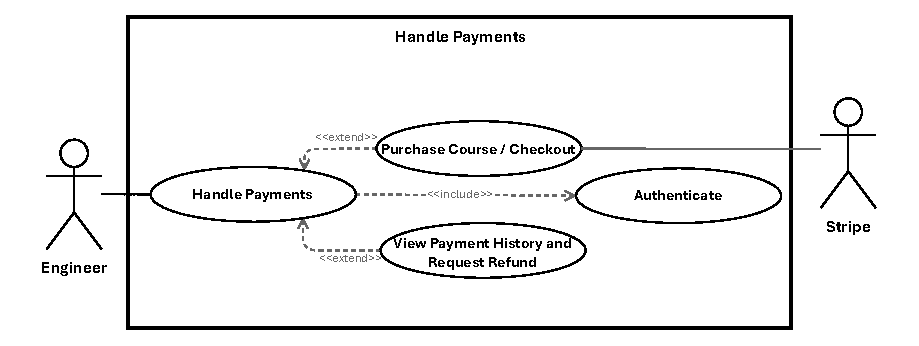
\includegraphics[width=\textwidth]{assets/chapter3/eng-handle-payments-use-case}
    \caption{Use Case Handle Payments}
    \label{fig:eng-handle-payments-use-case}
\end{figure}
\dotsection{\textbf{Specification of the Use Case Purchase Course / Checkout}}
\begin{table}[H]
    \centering
    \caption{Use Case Specification: Purchase Course / Checkout}
    \begin{tabular}{|p{3.5cm}|p{10.5cm}|}
        \hline
        \textbf{Title}          & Purchase Course / Checkout \\
        \hline
        \textbf{Summary}        & Engineer purchases a paid training path through Stripe checkout and is directed to a confirmation or cancellation screen depending on the outcome \\
        \hline
        \textbf{Primary Actor}  & Engineer \\
        \hline
        \textbf{Secondary Actor}& Stripe \\
        \hline
        \textbf{Precondition}   & The engineer has selected a training path for enrollment and has a valid payment method \\
        \hline
        \textbf{Post-condition} & Payment is confirmed and enrollment is activated, or the checkout is cancelled and no enrollment or payment record is created \\
        \hline
        \textbf{Basic Scenario} & \begin{minipage}[t]{\linewidth}
            \begin{enumerate}[topsep=0pt,itemsep=1pt,parsep=0pt,partopsep=0pt]
                \item Engineer reviews the training path details and price, then initiates checkout
                \item System redirects the engineer to the Stripe payment page
                \item For \textbf{Success}: engineer enters payment details and confirms; Stripe processes the payment and sends a webhook confirmation; system activates the enrollment, generates a receipt, and displays a confirmation screen with transaction details and a link to the training path
                \item For \textbf{Cancellation}: engineer aborts on the Stripe page; Stripe redirects to the platform cancellation screen; system displays a cancellation notice and offers options to retry checkout or return to the training path details; no payment or enrollment record is created
            \end{enumerate}
        \end{minipage} \\
        \hline
        \textbf{Error Scenario} & \begin{minipage}[t]{\linewidth}
            \begin{enumerate}[topsep=0pt,itemsep=1pt,parsep=0pt,partopsep=0pt]
                \item If the payment is declined, system displays the rejection reason
                \item If the webhook is not received, system polls Stripe for status
                \item If the training path price changed during checkout, system requests re-confirmation
                \item If enrollment activation is delayed after successful payment, system shows a processing message
                \item If the Stripe redirect fails in either direction, engineer may need to manually navigate back to the platform
            \end{enumerate}
        \end{minipage} \\
        \hline
    \end{tabular}
    \label{tab:eng-checkout}
\end{table}
\dotsection{\textbf{Specification of the Use Case View Payment History and Request Refund}}
\begin{table}[H]
    \centering
    \caption{Use Case Specification: View Payment History and Request Refund}
    \begin{tabular}{|p{3.5cm}|p{10.5cm}|}
        \hline
        \textbf{Title}          & View Payment History and Request Refund \\
        \hline
        \textbf{Summary}        & Engineer reviews past payment transactions and submits a refund request for an eligible purchase \\
        \hline
        \textbf{Actor}          & Engineer \\
        \hline
        \textbf{Precondition}   & The engineer is authenticated and has at least one completed payment transaction \\
        \hline
        \textbf{Post-condition} & Engineer has reviewed their transaction history, or a refund request is created with pending status and submitted for administrative review \\
        \hline
        \textbf{Basic Scenario} & \begin{minipage}[t]{\linewidth}
            \begin{enumerate}[topsep=0pt,itemsep=1pt,parsep=0pt,partopsep=0pt]
                \item Engineer navigates to the payment history section; system displays all transactions with date, training path, amount, and status; engineer may filter by date range or status
                \item Engineer selects a transaction to view its details
                \item For \textbf{Refund}: engineer clicks the refund option on an eligible transaction; system displays refund eligibility and a request form; engineer provides a reason and submits; system creates a pending refund request, notifies administrators for review, and allows the engineer to track the request status
            \end{enumerate}
        \end{minipage} \\
        \hline
        \textbf{Error Scenario} & \begin{minipage}[t]{\linewidth}
            \begin{enumerate}[topsep=0pt,itemsep=1pt,parsep=0pt,partopsep=0pt]
                \item If no payment history exists, system displays an empty state
                \item If the selected transaction is not eligible for a refund, system displays the refund policy
                \item If a refund request already exists for the transaction, system shows its current status
            \end{enumerate}
        \end{minipage} \\
        \hline
    \end{tabular}
    \label{tab:eng-payment-history}
\end{table}
\iffalse
\dotsection{\textbf{Specification of the Use Case Purchase Course / Checkout}}
\begin{table}[H]
    \centering
    \caption{Use Case Specification: Purchase Course / Checkout}
    \begin{tabular}{|p{3.5cm}|p{10.5cm}|}
        \hline
        \textbf{Title}          & Purchase Course / Checkout                                                                    \\
        \hline
        \textbf{Summary}        & Engineer purchases a training path, with payment processed via Stripe                   \\
        \hline
        \textbf{Primary Actor}  & Engineer                                                                                 \\
        \hline
        \textbf{Secondary Actor}& Stripe                                                                                 \\
        \hline
        \textbf{Precondition}   & The engineer has selected a training path for enrollment and has a valid payment method \\
        \hline
        \textbf{Post-condition} & Payment is confirmed, enrollment is activated, and a receipt is generated               \\
        \hline
        \textbf{Basic Scenario} & \begin{minipage}[t]{\linewidth}
                                      \begin{enumerate}[topsep=0pt,itemsep=1pt,parsep=0pt,partopsep=0pt]
                                          \item Engineer reviews the training path details and price
                                          \item Engineer initiates checkout and is redirected to Stripe payment
                                          \item Engineer enters payment details and confirms the transaction
                                          \item Stripe processes the payment and sends a webhook confirmation
                                          \item System activates the enrollment and generates a receipt
                                          \item Engineer receives confirmation and access to the training path
                                      \end{enumerate}
                                  \end{minipage}            \\
        \hline
        \textbf{Error Scenario} & \begin{minipage}[t]{\linewidth}
                                      \begin{enumerate}[topsep=0pt,itemsep=1pt,parsep=0pt,partopsep=0pt]
                                          \item If the payment is declined, the system displays the rejection reason
                                          \item If the webhook is not received, the system polls Stripe for status
                                          \item If the training path price changed during checkout, the system requests
                                                re-confirmation
                                      \end{enumerate}
                                  \end{minipage}    \\
        \hline
    \end{tabular}
    \label{tab:eng-checkout}
\end{table}
\dotsection{\textbf{Specification of the Use Case View Payment Success Result Screen}}
\begin{table}[H]
    \centering
    \caption{Use Case Specification: View Payment Success Result Screen}
    \begin{tabular}{|p{3.5cm}|p{10.5cm}|}
        \hline
        \textbf{Title}          & View Payment Success Result Screen                                                                 \\
        \hline
        \textbf{Summary}        & Engineer views the confirmation screen after successful payment completion                 \\
        \hline
        \textbf{Actor}          & Engineer                                                                                         \\
        \hline
        \textbf{Precondition}   & Payment has been successfully processed through Stripe                                         \\
        \hline
        \textbf{Post-condition} & Engineer sees payment confirmation and can access the enrolled training path                   \\
        \hline
        \textbf{Basic Scenario} & \begin{minipage}[t]{\linewidth}
                                      \begin{enumerate}[topsep=0pt,itemsep=1pt,parsep=0pt,partopsep=0pt]
                                          \item Engineer completes payment on Stripe checkout page
                                          \item Stripe redirects engineer to the platform success page
                                          \item System displays payment confirmation with transaction details
                                          \item System shows enrollment activation status
                                          \item Engineer can navigate to the training path or view receipt
                                      \end{enumerate}
                                  \end{minipage} \\
        \hline
        \textbf{Error Scenario} & \begin{minipage}[t]{\linewidth}
                                      \begin{enumerate}[topsep=0pt,itemsep=1pt,parsep=0pt,partopsep=0pt]
                                          \item If the redirect fails, engineer may need to manually navigate to the training path
                                          \item If enrollment activation is delayed, the system shows a processing message
                                      \end{enumerate}
                                  \end{minipage} \\
        \hline
    \end{tabular}
    \label{tab:eng-payment-success}
\end{table}
\dotsection{\textbf{Specification of the Use Case View Payment Cancelled Result Screen}}
\begin{table}[H]
    \centering
    \caption{Use Case Specification: View Payment Cancelled Result Screen}
    \begin{tabular}{|p{3.5cm}|p{10.5cm}|}
        \hline
        \textbf{Title}          & View Payment Cancelled Result Screen                                                                 \\
        \hline
        \textbf{Summary}        & Engineer views the cancellation screen after aborting the payment process                  \\
        \hline
        \textbf{Actor}          & Engineer                                                                                             \\
        \hline
        \textbf{Precondition}   & Payment was initiated but cancelled by the engineer on the Stripe checkout page              \\
        \hline
        \textbf{Post-condition} & Engineer sees cancellation confirmation and can retry or abandon the purchase               \\
        \hline
        \textbf{Basic Scenario} & \begin{minipage}[t]{\linewidth}
                                      \begin{enumerate}[topsep=0pt,itemsep=1pt,parsep=0pt,partopsep=0pt]
                                          \item Engineer initiates checkout but cancels on Stripe page
                                          \item Stripe redirects engineer to the platform cancellation page
                                          \item System displays cancellation confirmation
                                          \item System offers options to retry checkout or return to training path details
                                          \item No enrollment or payment record is created
                                      \end{enumerate}
                                  \end{minipage} \\
        \hline
        \textbf{Error Scenario} & \begin{minipage}[t]{\linewidth}
                                      \begin{enumerate}[topsep=0pt,itemsep=1pt,parsep=0pt,partopsep=0pt]
                                          \item If the redirect fails, engineer may need to manually navigate back to the training path
                                      \end{enumerate}
                                  \end{minipage} \\
        \hline
    \end{tabular}
    \label{tab:eng-payment-cancelled}
\end{table}
\dotsection{\textbf{Specification of the Use Case View Payment History}}
\begin{table}[H]
    \centering
    \caption{Use Case Specification: View Payment History}
    \begin{tabular}{|p{3.5cm}|p{10.5cm}|}
        \hline
        \textbf{Title}          & View Payment History                                                                 \\
        \hline
        \textbf{Summary}        & Engineer reviews their past payment transactions and refund requests                 \\
        \hline
        \textbf{Actor}          & Engineer                                                                              \\
        \hline
        \textbf{Precondition}   & The engineer is authenticated and has at least one payment transaction               \\
        \hline
        \textbf{Post-condition} & Engineer views a list of past payments with dates, amounts, and statuses             \\
        \hline
        \textbf{Basic Scenario} & \begin{minipage}[t]{\linewidth}
                                      \begin{enumerate}[topsep=0pt,itemsep=1pt,parsep=0pt,partopsep=0pt]
                                          \item Engineer navigates to the payment history section
                                          \item System retrieves all payment transactions for the engineer
                                          \item System displays payments with date, training path, amount, and status
                                          \item Engineer can filter by date range or status
                                          \item Engineer can view details of individual transactions
                                      \end{enumerate}
                                  \end{minipage}  \\
        \hline
        \textbf{Error Scenario} & \begin{minipage}[t]{\linewidth}
                                      \begin{enumerate}[topsep=0pt,itemsep=1pt,parsep=0pt,partopsep=0pt]
                                          \item If no payment history exists, the system displays an empty-state message
                                      \end{enumerate}
                                  \end{minipage} \\
        \hline
    \end{tabular}
    \label{tab:eng-payment-history}
\end{table}
\dotsection{\textbf{Specification of the Use Case Request Refund}}
\begin{table}[H]
    \centering
    \caption{Use Case Specification: Request Refund}
    \begin{tabular}{|p{3.5cm}|p{10.5cm}|}
        \hline
        \textbf{Title}          & Request Refund                                                                 \\
        \hline
        \textbf{Summary}        & Engineer submits a refund request for a paid training path purchase               \\
        \hline
        \textbf{Actor}          & Engineer                                                                        \\
        \hline
        \textbf{Precondition}   & The engineer has a completed payment transaction that meets refund eligibility     \\
        \hline
        \textbf{Post-condition} & A refund request is created and submitted for administrative review             \\
        \hline
        \textbf{Basic Scenario} & \begin{minipage}[t]{\linewidth}
                                      \begin{enumerate}[topsep=0pt,itemsep=1pt,parsep=0pt,partopsep=0pt]
                                          \item Engineer navigates to payment history
                                          \item Engineer selects a payment transaction
                                          \item System displays refund eligibility and request form
                                          \item Engineer provides reason for refund and submits request
                                          \item System creates refund request with pending status
                                          \item System notifies administrators for review
                                          \item Engineer can track refund request status
                                      \end{enumerate}
                                  \end{minipage}  \\
        \hline
        \textbf{Error Scenario} & \begin{minipage}[t]{\linewidth}
                                      \begin{enumerate}[topsep=0pt,itemsep=1pt,parsep=0pt,partopsep=0pt]
                                          \item If the payment is not eligible for refund, the system displays the policy
                                          \item If a refund request already exists, the system shows the current status
                                      \end{enumerate}
                                  \end{minipage} \\
        \hline
    \end{tabular}
    \label{tab:eng-refund}
\end{table}
\fi

\subsubsubsection[Manage Account]{Refinement of the Use Case Manage Account} Figure
\ref{fig:eng-manage-account-use-case} presents the refinement of the
Use Case Manage Account for the Engineer actor. This use case includes
the following sub-use cases:
\begin{figure}[H]
    \centering
    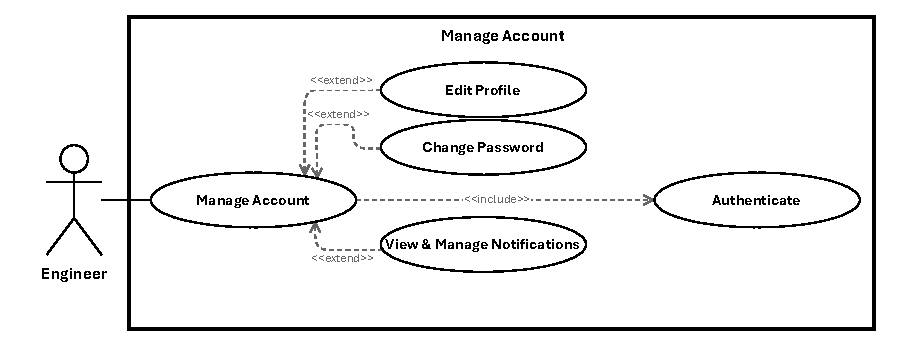
\includegraphics[width=\textwidth]{assets/chapter3/eng-manage-account-use-case}
    \caption{Use Case Manage Account}
    \label{fig:eng-manage-account-use-case}
\end{figure}
\dotsection{\textbf{Specification of the Use Case Edit Profile}}
\begin{table}[H]
    \centering
    \caption{Use Case Specification: Edit Profile}
    \begin{tabular}{|p{3.5cm}|p{10.5cm}|}
        \hline
        \textbf{Title}          & Edit Profile                                                                 \\
        \hline
        \textbf{Summary}        & Engineer updates their personal profile information including name, bio, and preferences \\
        \hline
        \textbf{Actor}          & Engineer                                                                      \\
        \hline
        \textbf{Precondition}   & The engineer is authenticated                                                  \\
        \hline
        \textbf{Post-condition} & Profile information is updated and persisted                                  \\
        \hline
        \textbf{Basic Scenario} & \begin{minipage}[t]{\linewidth}
                                      \begin{enumerate}[topsep=0pt,itemsep=1pt,parsep=0pt,partopsep=0pt]
                                          \item Engineer navigates to profile settings
                                          \item System displays current profile information
                                          \item Engineer updates name, bio, or other profile fields
                                          \item System validates the updated information
                                          \item System persists the changes
                                          \item Profile is updated across the platform
                                      \end{enumerate}
                                  \end{minipage}  \\
        \hline
        \textbf{Error Scenario} & \begin{minipage}[t]{\linewidth}
                                      \begin{enumerate}[topsep=0pt,itemsep=1pt,parsep=0pt,partopsep=0pt]
                                          \item If validation fails, the system displays specific error messages
                                          \item If update fails, the system preserves the previous profile data
                                      \end{enumerate}
                                  \end{minipage} \\
        \hline
    \end{tabular}
    \label{tab:eng-edit-profile}
\end{table}
\dotsection{\textbf{Specification of the Use Case Change Password}}
\begin{table}[H]
    \centering
    \caption{Use Case Specification: Change Password}
    \begin{tabular}{|p{3.5cm}|p{10.5cm}|}
        \hline
        \textbf{Title}          & Change Password                                                                 \\
        \hline
        \textbf{Summary}        & Engineer changes their account password for security purposes                      \\
        \hline
        \textbf{Actor}          & Engineer                                                                        \\
        \hline
        \textbf{Precondition}   & The engineer is authenticated and knows their current password                   \\
        \hline
        \textbf{Post-condition} & The password is updated and the engineer must authenticate with the new password \\
        \hline
        \textbf{Basic Scenario} & \begin{minipage}[t]{\linewidth}
                                      \begin{enumerate}[topsep=0pt,itemsep=1pt,parsep=0pt,partopsep=0pt]
                                          \item Engineer navigates to password settings
                                          \item System displays password change form
                                          \item Engineer enters current password
                                          \item Engineer enters new password and confirms it
                                          \item System validates current password and new password requirements
                                          \item System updates the password hash
                                          \item System confirms the change and may require re-authentication
                                      \end{enumerate}
                                  \end{minipage}  \\
        \hline
        \textbf{Error Scenario} & \begin{minipage}[t]{\linewidth}
                                      \begin{enumerate}[topsep=0pt,itemsep=1pt,parsep=0pt,partopsep=0pt]
                                          \item If current password is incorrect, the system rejects the change
                                          \item If new password does not meet requirements, the system displays validation errors
                                          \item If passwords do not match, the system prompts for confirmation
                                      \end{enumerate}
                                  \end{minipage} \\
        \hline
    \end{tabular}
    \label{tab:eng-change-password}
\end{table}
\dotsection{\textbf{Specification of the Use Case View \& Manage Notifications}}
\begin{table}[H]
    \centering
    \caption{Use Case Specification: View \& Manage Notifications}
    \begin{tabular}{|p{3.5cm}|p{10.5cm}|}
        \hline
        \textbf{Title}          & View \& Manage Notifications                                                                 \\
        \hline
        \textbf{Summary}        & Engineer views system notifications and manages their read/unread status            \\
        \hline
        \textbf{Actor}          & Engineer                                                                                   \\
        \hline
        \textbf{Precondition}   & The engineer is authenticated and has received notifications                           \\
        \hline
        \textbf{Post-condition} & Engineer views notifications and can mark them as read or take actions                \\
        \hline
        \textbf{Basic Scenario} & \begin{minipage}[t]{\linewidth}
                                      \begin{enumerate}[topsep=0pt,itemsep=1pt,parsep=0pt,partopsep=0pt]
                                          \item Engineer navigates to notifications section
                                          \item System displays list of notifications with read/unread status
                                          \item System shows notification type, content, and timestamp
                                          \item Engineer can click a notification to view details
                                          \item Engineer can mark notifications as read or unread
                                          \item Engineer can dismiss or delete notifications
                                      \end{enumerate}
                                  \end{minipage}  \\
        \hline
        \textbf{Error Scenario} & \begin{minipage}[t]{\linewidth}
                                      \begin{enumerate}[topsep=0pt,itemsep=1pt,parsep=0pt,partopsep=0pt]
                                          \item If no notifications exist, the system displays an empty-state message
                                      \end{enumerate}
                                  \end{minipage} \\
        \hline
    \end{tabular}
    \label{tab:eng-notifications}
\end{table}